\section{Wykaz zmiennych pomocniczych rozważanych w podejściu obszarowym}

\begin{itemize}
\item gęstość zaludnienia
\item wskaźnik zależności osób w wieku przedprodukcyjnym i poprodukcyjnym w odniesieniu do liczby osób w wieku produkcyjnym
\item wskaźnik zależności osób w wieku przedprodukcyjnym w odniesieniu do liczby osób w wieku produkcyjnym
\item wskaźnik zależności osób w wieku poprodukcyjnym w odniesieniu do liczby osób w wieku produkcyjnym
\item udział liczby osób na wsi w ludności ogółem
\item udział liczby osób w miastach w ludności ogółem
\item współczynnik aktywności zawodowej ogółem
\item wskaźnik zatrudnienia ogółem
\item stopa bezrobocia ogółem
\item udział osób w gospodarstwach domowych korzystających ze środowiskowej pomocy społecznej w ludności ogółem
\item udział osób w wieku przedprodukcyjnym w gospodarstwach domowych korzystających ze środowiskowej pomocy społecznej w ogólnej liczbie osób w tym wieku
\item udział osób w wieku produkcyjnym w gospodarstwach domowych korzystających ze środowiskowej pomocy społecznej w ogólnej liczbie osób w tym wieku
\item udział osób w wieku poprodukcyjnym w gospodarstwach domowych korzystających ze środowiskowej pomocy społecznej w ogólnej liczbie osób w tym wieku
\item udział dzieci w wieku do lat 17, na które rodzice otrzymują zasiłek rodzinny w ogólnej liczbie dzieci w tym wieku
\item udział rodzin samotnie wychowujących co najmniej jedno dziecko w liczbie rodzin ogółem
\item przeciętna liczba dzieci do lat 24 na utrzymaniu w rodzinach
\item udział rodzin z co najmniej jednym dzieckiem do lat 24 pozostającym na utrzymaniu w~liczbie rodzin ogółem
\item udział rodzin z 3 dzieci do lat 24 pozostającymi na utrzymaniu w liczbie rodzin ogółem
\item udział rodzin z 3 i więcej dzieci do lat 24 pozostającymi na utrzymaniu w liczbie rodzin ogółem
\item udział rodzin z 4 i więcej dzieci do lat 24 pozostającymi na utrzymaniu w liczbie rodzin ogółem
\item udział osób z wykształceniem zasadniczym zawodowym w liczbie osób w wieku 20--64 lata
\item udział osób z wykształceniem zasadniczym zawodowym w liczbie osób w wieku 20--64 lata (logarytm)
\item udział osób z wykształceniem wyższym w liczbie osób w wieku 25--64 lata
\item udział osób z wykształceniem podstawowym nieukończonym i bez wykształcenia w liczbie osób ogółem
\item przeciętna liczba osób w gospodarstwie domowym
\item udział gospodarstw domowych czterooosobowych w liczbie gospodarstw ogółem
\item udział gospodarstw domowych pięcio i więcej osobowych w liczbie gospodarstw ogółem
\item udział liczby osób w mieszkaniach, gdzie przypada powyżej 3 osób na izbę w~ludności w~mieszkaniach zamieszkałych stale ogółem
\item udział liczby mieszkań, gdzie przypada powyżej 3 osób na izbę w liczbie mieszkań ogółem
\item udział ludności w mieszkaniach zamieszkałych stale wyposażonych w~łazienkę w~ludności w~mieszkaniach zamieszkałych stale ogółem
\item udział ludności w mieszkaniach zamieszkałych stale wyposażonych w ustęp spłukiwany w~ludności w mieszkaniach zamieszkałych stale ogółem
\item udział ludności w mieszkaniach zamieszkałych stale wyposażonych w ciepłą wodę bieżącą w ludności w mieszkaniach zamieszkałych stale ogółem
\item udział ludności w mieszkaniach zamieszkałych stale bez wodociągu w ludności w mieszkaniach zamieszkałych stale ogółem
\item udział osób utrzymujących się z renty w liczbie osób ogółem
\item udział osób utrzymujących się z pracy w rolnictwie w liczbie osób ogółem
\item udział osób utrzymujących się z pozostałych źródeł w liczbie osób ogółem
\item udział osób w wieku 20-29 lat utrzymywanych w liczbie osób ogółem
\item udział osób w wieku 20--29 lat utrzymywanych w liczbie osób  w wieku 20--29 lat
\item udział osób w wieku 30-39 lat utrzymywanych w liczbie osób ogółem
\item udział osób w wieku 30--39 lat utrzymywanych w liczbie osób  w wieku 30--39 lat
\item udział osób w wieku 65 lat i więcej utrzymująca się z renty w liczbie osób w wieku 65 lat i~więcej
\item udział osób w wieku 65 lat i więcej utrzymująca się z pozostałych źródeł w liczbie osób w~wieku 65 lat i więcej
\item udział osób niepełnosprawnych prawnie w liczbie osób ogółem
\item udział osób niepełnosprawnych prawnie w liczbie osób niepełnosprawnych ogółem
\item udział osób niepełnosprawnych biologicznie w liczbie osób ogółem
\item udział osób niepełnosprawnych biologicznie w liczbie osób niepełnosprawnych ogółem
\item stopa bezrobocia rejestrowanego
\item udział bezrobotnych zarejestrowanych w liczbie ludności w wieku produkcyjnym
\item udział bezrobotnych zarejestrowanych powyżej 12 miesięcy bez pracy w liczbie osób pracujących i bezrobotnych
\item udział bezrobotnych zarejestrowanych powyżej 24 miesięcy bez pracy w liczbie osób pracujących i bezrobotnych
\item przeciętne miesięczne wynagrodzenie brutto
\item zgony z powodu nowotworów ogółem na 100 tys. ludności
\item zgony osób z powodu chorób układu krążenia na 100 tys. ludności
\end{itemize}

\newpage

\section{Kody R}

\subsection*{Bootstrap dla modelu Faya-Herriota z uwzględnieniem transformacji zmiennej zależnej}

\begin{verbatim}
fh_bootstrap <- function(m, psi, beta, sigma, x, B, trans = F){

  bias <- matrix(0, m, B)
  mse <- matrix(0, m, B)
  
  for(i in 1:B){
    
    u_g <- rnorm(m, 0, sqrt(sigma))
    e_g <- rnorm(m, 0, sqrt(psi))
     
    theta_g <- x%*%beta + u_g
    direct_g <- theta_g + e_g
    
    FH_g=eblupFH(direct_g~x-1, psi)
    
    eblup <- FH_g$eblup
    
    if(trans == T){
      eblup <- arcsin_trans(eblup, inv = T)
      theta_g <- arcsin_trans(theta_g, inv = T)
    }
    
    bias[,i] <- eblup - theta_g
    mse[,i] <- (eblup - theta_g)^2
    
  }
  
  results <- list(mse = rowMeans(mse),
                  bias = rowMeans(bias))
  return(results) 
}
\end{verbatim}

\subsection*{Bootstrap dla przestrzennego modelu Faya-Herriota z uwzględnieniem transformacji zmiennej zależnej}

\begin{verbatim}
sfh_bootstrap <- function(m, psi, beta, sigma, rho, nbq, x, B, trans = F){
    
  bias <- matrix(0, m, B)
  mse <- matrix(0, m, B)
  v <- solve(diag(m)-rho*nbq)
  
  for(i in 1:B){
    
    # cat("B =",i, "\n")
    
    u_g <- rnorm(m, 0, sqrt(sigma))
    e_g <- rnorm(m, 0, sqrt(psi))
    
    theta_g <- x%*%beta + v%*%u_g
    direct_g <- theta_g + e_g
     
    SFH_g=eblupSFH(direct_g~x-1, psi, nbq)
       
    eblup <- SFH_g$eblup
    
    if(trans == T){
      eblup <- arcsin_trans(eblup, inv = T)
      theta_g <- arcsin_trans(theta_g, inv = T)
    }
    
    bias[,i] <- eblup - theta_g
    mse[,i] <- (eblup - theta_g)^2
    
  }
  
  results <- list(mse = rowMeans(mse),
                  bias = rowMeans(bias))
  return(results)
  
}
\end{verbatim}

\subsection*{Estymator EB uwzględniający liczbę osób w gospodarstwie oraz wielowątkowość procesora}

\begin{verbatim}
eb1 <- function(eq, census, surv, lvl1, MC=100, shift, lam=0, povline){
  
  formula <- eq
  
  r_d1 <- census %>%
    group_by_(lvl1) %>%
    summarise(rd1=n())
  
  s_d1 <- surv %>%
    group_by_(lvl1) %>%
    summarise(sd1=n()) 
  
  formuladata <- model.frame(formula, na.action = na.omit, data=surv)
  Xs <- model.matrix(formula, data=surv)
  
  m <- shift
  y <- formuladata[, 1]
  y_m <- y + m
  y_log <- bxcx(y_m, lambda = lam, type = "BoxCox")
  
  lvl1_s <- surv[,lvl1]
  lvl1_r <- unique(census[,lvl1])
  d1 <- length(lvl1_r)
  
  fit.EB <- lmer(formula = y_log ~ (1 | lvl1_s) + -1 + Xs)
  # summary(fit.EB)
  
  betaest <- matrix(fixed.effects(fit.EB), nrow = ncol(formuladata), ncol = 1)
  upred_d1 <- data.frame(lvl1=s_d1[lvl1],
                         upred_d1=random.effects(fit.EB)$lvl1_s)
  
  names(upred_d1)[2] <- "upred_d1"
  
  sigmae2est <- as.data.frame(VarCorr(fit.EB))[2,4]
  sigmau2est_d1 <- as.data.frame(VarCorr(fit.EB))[1,4]
  sqrtsigmae2est <- sqrt(sigmae2est)
  
  rs_d1 <- left_join(r_d1,left_join(s_d1,upred_d1, by=lvl1), by=lvl1)
  rs_d1[is.na(rs_d1)] <- 0
  
  rs <- rs_d1 %>%
    as.matrix()
  
  Xr <- census %>%
    mutate(intercept=1) %>%
    select(get(lvl1), intercept, l_mez_os:lau1_benefits)
  
  Resultsfit <- list(summary = summary(fit.EB), 
                     fixed = fixed.effects(fit.EB),
                     random_d1 = upred_d1,
                     errorvar = sigmae2est,
                     refvar_d1 = sigmau2est_d1,
                     residuals = residuals(fit.EB),
                     rs = rs)
  
  povrate <- function(y) {
    z <- povline
    result <- mean(y<z)
    return (result)
  }
  
  povgap <- function(y)     
  {
    z <- povline
    result <- mean((y<z) * (z-y) / z) 
    return (result)
  }
  
  eb_lvl1 <- function(i){
    
    Xr_i <- Xr[Xr[,lvl1]==lvl1_r[i],]
    
    yb_i <- as.matrix(Xr_i[,2:ncol(Xr_i)]) %*% as.numeric(betaest)
    
    ud1_i <- as.numeric(rs[rs[,lvl1]==lvl1_r[i],"upred_d1"])
    
    sd1_i <- as.numeric(rs[rs[,lvl1]==lvl1_r[i],"sd1"])
    
    mudpred <- yb_i + ud1_i
    
    sqrtsigmav2_d1=sqrt(sigmau2est_d1 * (1 - sigmau2est_d1/
    	(sigmau2est_d1 + sigmae2est/sd1_i)))
    
    ysd <- surv[surv[,lvl1]==lvl1_r[i],names(formuladata)[1]] + m
    
    h_surv <- surv[surv[,lvl1]==lvl1_r[i],"l_os"]
    h_cens <- census[census[,lvl1]==lvl1_r[i],"l_os"]
    h <- c(h_cens, h_surv)

    if(length(ysd)!=0){
      ysd_log <- bxcx(ysd, lambda = 0, type = "BoxCox")
    } else{
      ysd_log <- ysd
    }
    
    ed <- sapply(1:MC, function(k){
      l <- length(mudpred)
      ud1_ell <- rnorm(1, 0, sqrtsigmav2_d1)
      ed_ell <- rnorm(l, 0, sqrtsigmae2est)
      yrdpred <- mudpred + ud1_ell + ed_ell
      ydnew <- c(yrdpred, ysd_log)
      Ednew <- bxcx(ydnew, lambda = lam, type = "BoxCox", InverseQ = TRUE) - m
      Ednew_h <- rep.int(Ednew, h)
      return(povrate(Ednew_h))
    })
    
    return(ed)
  }
  
  eb <- foreach(i=1:length(lvl1_r), .combine="rbind") %do% {
    eb_lvl1(i)
  }
  
  pov_lvl1 <- apply(eb, 1, mean)
  
  lvl1_eb <- data.frame(lvl1=lvl1_r, eb=pov_lvl1)
  
  result <- list(eb=lvl1_eb, model=Resultsfit)
  
  return(result)
}
\end{verbatim}

\subsection*{Estymator MSE dla metody EB uwzględniający liczbę osób w gospodarstwie oraz wielowątkowość procesora}

\begin{verbatim}
mse1 <- function(eq, census, surv, lvl1, MC=100, B=100, shift, lam=0, povline){
  
  formula <- eq
  
  wyniki_lvl1 <- eb1(eq=formula, census=census, surv=surv, lvl1=lvl1, MC=MC, 
  	shift=shift, lam=lam, povline=povline)
  
  Xs <- model.matrix(formula, data=surv)
  
  Xr <- census %>%
    mutate(intercept=1) %>%
    select(get(lvl1), intercept, l_mez_os:lau1_benefits)
  
  musd.B <- as.numeric(Xs %*% wyniki_lvl1$model$fixed)
  murd.B <- as.matrix(Xr[,2:ncol(Xr)]) %*% as.numeric(wyniki_lvl1$model$fixed)
  
  sqrtsigmae2est <- sqrt(wyniki_lvl1$model$errorvar)
  sqrtsigmav2_d1 <- sqrt(wyniki_lvl1$model$refvar_d1)
  
  # pętla bootstrap
  
  povrate <- function(y) {
    z <- povline
    result <- mean(y<z)
    return (result)
  }
  
  povgap <- function(y)     
  {
    z <- povline
    result <- mean((y<z) * (z-y) / z) 
    return (result)
  }
  
  mse_eb <- function(b){
    
    cat("B = ",b,"\n")
    
    lvl1_s <- surv[,lvl1]
    
    lvl1_su <- unique(lvl1_s)
    
    mus.B <- data.frame(lvl1_s, musd.B)
    
    ys.B_lvl1 <- function(i){
      
      musd.B_i <- mus.B[mus.B[,"lvl1_s"]==lvl1_su[i],]
      l <- nrow(musd.B_i)
      ed.B <- rnorm(l, 0, sqrtsigmae2est)
      ud1.B <- rnorm(1, 0, sqrtsigmav2_d1)
      ys.B <- musd.B_i[,"musd.B"] + ud1.B + ed.B
      
      ysB.df <- data.frame(lvl1=lvl1_su[i],
                           ys.B, ud1.B)
      
      return(ysB.df)
      
    }
    
    ys.B <- foreach(i=1:length(lvl1_su), .combine="rbind") %do% {
      ys.B_lvl1(i)
    }
    
    m <- shift
    
    Es.B <- bxcx(ys.B$ys.B, lambda = lam, type = "BoxCox", InverseQ = TRUE) - m
    
    survB <- cbind(surv, Es.B)
    
    formulaB <- Es.B ~ l_mez_os+l_30_44_os+l_65_w_os+
      l_bezr_os+l_niep_os+l_wyk_pod_os+l_wyk_wyz_os+
      pok_1+pok_3_w+mw_wies+ob_dzieci+lau1_unempl+lau1_nace_a+lau1_benefits
    
    ebB <- eb1(eq=formulaB, census=census, surv=survB, lvl1=lvl1, MC=MC, 
    	shift=shift, lam=lam, povline=povline)
    
    lvl1_r <- Xr[,lvl1]
    
    mur.B <- data.frame(lvl1_r, murd.B)
    
    lvl1_ru <- unique(lvl1_r)
    
    rs <- wyniki_lvl1$model$rs
    
    udB <- ys.B %>%
      select(-ys.B) %>%
      distinct() %>%
      as.matrix()
    
    mse_lvl1 <- function(i){
      
      mur.B_i <- mur.B[mur.B[,"lvl1_r"]==lvl1_ru[i],"murd.B"]
      
      sd1_i <- as.numeric(rs[rs[,lvl1]==lvl1_ru[i],"sd1"])
      
      erd.B <- rnorm(length(mur.B_i), 0, sqrtsigmae2est)
      
      ud1B <- as.numeric(udB[udB[,"lvl1"]==lvl1_ru[i],"ud1.B"])
      
      if(sd1_i==0){
        yrd.B <- mur.B_i + rnorm(1, 0, sqrtsigmav2_d1) + erd.B
        Ed.B <- bxcx(yrd.B, lambda = lam, type = "BoxCox", InverseQ = TRUE) - m
      } else{
        yrd.B <- mur.B_i + ud1B + erd.B
        ysd.B <- mus.B[mus.B[,"lvl1_s"]==lvl1_ru[i],"musd.B"]
        yrsd.B <- c(yrd.B, ysd.B)
        Ed.B <- bxcx(yrsd.B, lambda = lam, type = "BoxCox", InverseQ = TRUE) - m
      }
      
      bias <- ebB$eb[i,"eb"] - povrate(Ed.B)
      mse <- (bias)^2
      
      res <- data.frame(bias=bias,
                        mse=mse)
      
      colnames(res) <- c(paste0("bias",b), paste0("mse",b))
      
      return(res)
    }
    
    mseB <- foreach(i=1:length(lvl1_ru), .combine="rbind") %do% {
      mse_lvl1(i)
    }
    
    return(mseB)
    
  }
  
  mse_fin <- foreach(b=1:B, .combine="cbind") %do% {
    mse_eb(b)
  }
  
  mse <- mse_fin %>%
    select(starts_with("mse")) %>%
    transmute(mse=rowMeans(.))
  
  bias <- mse_fin %>%
    select(starts_with("bias")) %>%
    transmute(bias=rowMeans(.))
  
  results <- cbind(wyniki_lvl1$eb, mse, bias)
  #results <- mse_fin
  
  return(results)
  
}
\end{verbatim}

\newpage

\section{Bezpośrednie i pośrednie oszacowania stopy oraz głębokości ubóstwa}

% stopa ubóstwa podreg
\begin{center}
\footnotesize
\begin{longtable}{p{6cm}rrrr}
\caption{Oszacowania stopy ubóstwa w podregionach w roku 2011 z wykorzystaniem estymatora bezpośredniego oraz SEBLUP wraz z wartością błędu standardowego}\\
\label{tab:podreg_hcr}\\
\hline
Nazwa podregionu & HT & SE(HT) & SEBLUP & SE(SEBLUP) \\
  \hline
\endfirsthead
  \hline
Nazwa podregionu & HT & SE(HT) & SEBLUP & SE(SEBLUP) \\
  \hline
\endhead
\hline \multicolumn{5}{|r|}{{Ciąg dalszy na następnej stronie}} \\
\hline
\endfoot
\hline
\endlastfoot
\hline
Podregion 1 - jeleniogórski              & 15,7    & 1,7         & 15,2     & 1,5          \\
Podregion 2 - legnicko-głogowski         & 14,4    & 1,9         & 15,2     & 1,6          \\
Podregion 3 - wałbrzyski                 & 15,3    & 1,5         & 16       & 1,5          \\
Podregion 4 - wrocławski                 & 11,3    & 1,6         & 11,4     & 1,4          \\
Podregion 5 - m. Wrocław                 & 6,2     & 1,2         & 6,2      & 1,2          \\
Podregion 6 - bydgosko-toruński          & 11,5    & 1,5         & 12,1     & 1,5          \\
Podregion 7 - grudziądzki                & 26,1    & 2,3         & 23,9     & 1,9          \\
Podregion 8 - włocławski                 & 18,3    & 1,6         & 18,1     & 1,6          \\
Podregion 9 - bialski                    & 35,2    & 3,2         & 34,8     & 2,4          \\
Podregion 10 - chełmsko-zamojski         & 34,7    & 1,8         & 33,7     & 1,6          \\
Podregion 11 - lubelski                  & 24      & 1,7         & 23,8     & 1,6          \\
Podregion 12 - puławski                  & 35,4    & 2,4         & 34,5     & 1,9          \\
Podregion 13 - gorzowski                 & 31      & 3,4         & 26,9     & 2,5          \\
Podregion 14 - zielonogórski             & 21,7    & 2,1         & 21,6     & 1,8          \\
Podregion 15 - łódzki                    & 14,1    & 2,1         & 15,2     & 1,8          \\
Podregion 16 - m. Łódź                   & 13,9    & 1,6         & 13,7     & 1,5          \\
Podregion 17 - piotrkowski               & 23,6    & 1,6         & 23       & 1,4          \\
Podregion 18 - sieradzki                 & 21,5    & 2,1         & 22,4     & 1,8          \\
Podregion 19 - skierniewicki             & 21,5    & 2,2         & 22,3     & 1,8          \\
Podregion 20 - krakowski                 & 17,7    & 1,7         & 18,3     & 1,5          \\
Podregion 21 - m. Kraków                 & 8,4     & 1,5         & 8,9      & 1,4          \\
Podregion 22 - nowosądecki               & 28,8    & 2,1         & 28,1     & 1,8          \\
Podregion 23 - oświęcimski               & 12      & 1,6         & 12,1     & 1,4          \\
Podregion 24 - tarnowski                 & 40,9    & 3           & 34,6     & 2,3          \\
Podregion 25 - ciechanowsko-płocki       & 18,2    & 1,6         & 18,3     & 1,4          \\
Podregion 26 - ostrołęcko-siedlecki      & 21,1    & 1,6         & 21,3     & 1,5          \\
Podregion 27 - radomski                  & 23,5    & 1,8         & 23,3     & 1,6          \\
Podregion 28 - m. Warszawa               & 6,2     & 0,9         & 6        & 0,8          \\
Podregion 29 - warszawski wschodni       & 12,8    & 1,3         & 13,2     & 1,2          \\
Podregion 30 - warszawski zachodni       & 10,8    & 1,3         & 11,1     & 1,2          \\
Podregion 31 - nyski                     & 12,2    & 2,2         & 13,3     & 1,9          \\
Podregion 32 - opolski                   & 14,2    & 1,8         & 12,8     & 1,5          \\
Podregion 33 - krośnieński               & 25,9    & 2,2         & 25,8     & 1,8          \\
Podregion 34 - przemyski                 & 28,6    & 2,6         & 27,9     & 2,1          \\
Podregion 35 - rzeszowski                & 14,7    & 1,5         & 15,5     & 1,3          \\
Podregion 36 - tarnobrzeski              & 19,7    & 2           & 20,3     & 1,7          \\
Podregion 37 - białostocki               & 12      & 1,7         & 12,2     & 1,6          \\
Podregion 38 - łomżyński                 & 21,4    & 2,9         & 23,4     & 2,2          \\
Podregion 39 - suwalski                  & 18,5    & 3,2         & 19,9     & 2,4          \\
Podregion 40 - gdański                   & 11      & 1,4         & 12,5     & 1,3          \\
Podregion 41 - słupski                   & 29,7    & 2,8         & 26,6     & 2,1          \\
Podregion 42 - starogardzki              & 17,3    & 2,1         & 17,8     & 1,8          \\
Podregion 43 - trójmiejski               & 13,3    & 1,9         & 11,4     & 1,8          \\
Podregion 44 - bielski                   & 10,5    & 1,1         & 10,7     & 1,1          \\
Podregion 45 - bytomski                  & 24,1    & 2,4         & 21,1     & 2,1          \\
Podregion 46 - częstochowski             & 15,2    & 1,6         & 15,3     & 1,4          \\
Podregion 47 - gliwicki                  & 13,4    & 1,8         & 14,3     & 1,6          \\
Podregion 48 - katowicki                 & 13,6    & 1,3         & 13,8     & 1,2          \\
Podregion 49 - rybnicki                  & 10,1    & 1,3         & 9,9      & 1,3          \\
Podregion 50 - sosnowiecki               & 9,5     & 1,2         & 9,6      & 1,2          \\
Podregion 51 - tyski                     & 10,3    & 1,5         & 10,3     & 1,4          \\
Podregion 52 - kielecki                  & 22,2    & 1,5         & 22,5     & 1,4          \\
Podregion 53 - sandomiersko-jędrzejowski & 34      & 2,8         & 30,8     & 2,2          \\
Podregion 54 - elbląski                  & 17,6    & 1,7         & 18,3     & 1,6          \\
Podregion 55 - ełcki                     & 17,5    & 2,9         & 18,5     & 2,3          \\
Podregion 56 - olsztyński                & 14,8    & 1,8         & 15,3     & 1,5          \\
Podregion 57 - kaliski                   & 17,5    & 1,5         & 17,1     & 1,3          \\
Podregion 58 - koniński                  & 21,3    & 2           & 20,8     & 1,7          \\
Podregion 59 - leszczyński               & 18      & 2           & 18,4     & 1,8          \\
Podregion 60 - pilski                    & 21,6    & 2,3         & 22,8     & 1,8          \\
Podregion 61 - poznański                 & 13,4    & 1,7         & 12,9     & 1,4          \\
Podregion 62 - m. Poznań                 & 7,7     & 1,7         & 8        & 1,5          \\
Podregion 63 - koszaliński               & 21,9    & 2,2         & 19,6     & 1,9          \\
Podregion 64 - stargardzki               & 17,3    & 3,2         & 20,2     & 2,4          \\
Podregion 65 - m. Szczecin               & 11,6    & 2,4         & 12,4     & 2            \\
Podregion 66 - szczeciński               & 16,5    & 2,6         & 15,3     & 2,1          \\   
\hline
\end{longtable}
\small{Źródło: opracowanie własne na podstawie badania EU-SILC 2011, NSP 2011 oraz BDL.}
\end{center}

% głębokość ubóstwa podreg
\begin{center}
\footnotesize
\begin{longtable}{p{6cm}rrrr}
\caption{Oszacowania głębokości ubóstwa w podregionach w roku 2011 z wykorzystaniem estymatora bezpośredniego oraz SEBLUP wraz z wartością błędu standardowego}\\
\label{tab:podreg_pgi}\\
\hline
Nazwa podregionu & HT & SE(HT) & SEBLUP & SE(SEBLUP) \\
  \hline
\endfirsthead
  \hline
Nazwa podregionu & HT & SE(HT) & SEBLUP & SE(SEBLUP) \\
  \hline
\endhead
\hline \multicolumn{5}{|r|}{{Ciąg dalszy na następnej stronie}} \\
\hline
\endfoot
\hline
\endlastfoot
\hline
Podregion 1 - jeleniogórski              & 5,1     & 0,7         & 5,1      & 0,6          \\
Podregion 2 - legnicko-głogowski         & 4,7     & 0,8         & 4,5      & 0,7          \\
Podregion 3 - wałbrzyski                 & 3,6     & 0,4         & 3,6      & 0,4          \\
Podregion 4 - wrocławski                 & 3,3     & 0,7         & 3,2      & 0,6          \\
Podregion 5 - m. Wrocław                 & 1,9     & 0,5         & 1,9      & 0,5          \\
Podregion 6 - bydgosko-toruński          & 2,4     & 0,5         & 2,7      & 0,5          \\
Podregion 7 - grudziądzki                & 6       & 0,7         & 5,5      & 0,6          \\
Podregion 8 - włocławski                 & 4,9     & 0,5         & 4,9      & 0,4          \\
Podregion 9 - bialski                    & 6,8     & 0,9         & 7,1      & 0,7          \\
Podregion 10 - chełmsko-zamojski         & 8,7     & 0,6         & 8,5      & 0,6          \\
Podregion 11 - lubelski                  & 6,7     & 0,6         & 6,5      & 0,6          \\
Podregion 12 - puławski                  & 8,6     & 0,7         & 8,4      & 0,6          \\
Podregion 13 - gorzowski                 & 7       & 0,9         & 6,2      & 0,7          \\
Podregion 14 - zielonogórski             & 5,3     & 0,8         & 5,2      & 0,7          \\
Podregion 15 - łódzki                    & 4,6     & 0,9         & 4,6      & 0,7          \\
Podregion 16 - m. Łódź                   & 4       & 0,6         & 4,1      & 0,5          \\
Podregion 17 - piotrkowski               & 5,7     & 0,5         & 5,9      & 0,5          \\
Podregion 18 - sieradzki                 & 7,6     & 0,9         & 7        & 0,8          \\
Podregion 19 - skierniewicki             & 5,3     & 0,8         & 5,2      & 0,7          \\
Podregion 20 - krakowski                 & 4,5     & 0,5         & 4,5      & 0,5          \\
Podregion 21 - m. Kraków                 & 2,4     & 0,6         & 2,5      & 0,6          \\
Podregion 22 - nowosądecki               & 12      & 1,1         & 10,7     & 0,9          \\
Podregion 23 - oświęcimski               & 3,5     & 0,6         & 3,7      & 0,5          \\
Podregion 24 - tarnowski                 & 10,4    & 1           & 9,1      & 0,8          \\
Podregion 25 - ciechanowsko-płocki       & 4,3     & 0,6         & 4,5      & 0,5          \\
Podregion 26 - ostrołęcko-siedlecki      & 5       & 0,5         & 5        & 0,4          \\
Podregion 27 - radomski                  & 6,8     & 0,6         & 6,7      & 0,6          \\
Podregion 28 - m. Warszawa               & 1,9     & 0,3         & 1,8      & 0,3          \\
Podregion 29 - warszawski wschodni       & 2,3     & 0,3         & 2,5      & 0,3          \\
Podregion 30 - warszawski zachodni       & 3,8     & 0,6         & 3,7      & 0,6          \\
Podregion 31 - nyski                     & 2,9     & 0,6         & 3,3      & 0,6          \\
Podregion 32 - opolski                   & 4,1     & 0,6         & 3,8      & 0,6          \\
Podregion 33 - krośnieński               & 5,8     & 0,6         & 5,9      & 0,6          \\
Podregion 34 - przemyski                 & 8       & 1           & 7,1      & 0,8          \\
Podregion 35 - rzeszowski                & 4,4     & 0,5         & 4,5      & 0,5          \\
Podregion 36 - tarnobrzeski              & 3,6     & 0,4         & 3,8      & 0,3          \\
Podregion 37 - białostocki               & 2,2     & 0,3         & 2,2      & 0,3          \\
Podregion 38 - łomżyński                 & 4,4     & 0,7         & 4,4      & 0,6          \\
Podregion 39 - suwalski                  & 2,5     & 0,5         & 2,6      & 0,5          \\
Podregion 40 - gdański                   & 3,6     & 0,6         & 3,9      & 0,5          \\
Podregion 41 - słupski                   & 5,6     & 0,7         & 5,5      & 0,6          \\
Podregion 42 - starogardzki              & 4,6     & 0,6         & 4,7      & 0,6          \\
Podregion 43 - trójmiejski               & 4,6     & 0,9         & 3,9      & 0,7          \\
Podregion 44 - bielski                   & 3,6     & 0,6         & 3,5      & 0,6          \\
Podregion 45 - bytomski                  & 6,4     & 0,9         & 5,6      & 0,7          \\
Podregion 46 - częstochowski             & 5,5     & 0,8         & 5,7      & 0,6          \\
Podregion 47 - gliwicki                  & 5,9     & 0,9         & 5,4      & 0,7          \\
Podregion 48 - katowicki                 & 5,3     & 0,6         & 5,2      & 0,6          \\
Podregion 49 - rybnicki                  & 2,5     & 0,4         & 2,5      & 0,4          \\
Podregion 50 - sosnowiecki               & 2,7     & 0,4         & 2,9      & 0,4          \\
Podregion 51 - tyski                     & 2,8     & 0,5         & 2,7      & 0,4          \\
Podregion 52 - kielecki                  & 6,4     & 0,6         & 6,7      & 0,6          \\
Podregion 53 - sandomiersko-jędrzejowski & 14,1    & 1,5         & 10,8     & 1            \\
Podregion 54 - elbląski                  & 2,6     & 0,4         & 2,7      & 0,4          \\
Podregion 55 - ełcki                     & 3       & 0,6         & 3,2      & 0,6          \\
Podregion 56 - olsztyński                & 5       & 0,7         & 4,8      & 0,7          \\
Podregion 57 - kaliski                   & 6,1     & 0,7         & 5,9      & 0,6          \\
Podregion 58 - koniński                  & 4,6     & 0,5         & 4,8      & 0,5          \\
Podregion 59 - leszczyński               & 3,9     & 0,7         & 3,9      & 0,6          \\
Podregion 60 - pilski                    & 6       & 0,8         & 5,7      & 0,7          \\
Podregion 61 - poznański                 & 2,4     & 0,5         & 2,4      & 0,4          \\
Podregion 62 - m. Poznań                 & 2,5     & 0,8         & 2,4      & 0,7          \\
Podregion 63 - koszaliński               & 6,5     & 1           & 6        & 0,7          \\
Podregion 64 - stargardzki               & 3,4     & 0,7         & 4        & 0,6          \\
Podregion 65 - m. Szczecin               & 2,7     & 0,6         & 2,8      & 0,6          \\
Podregion 66 - szczeciński               & 5,1     & 1,1         & 4,5      & 0,9          \\
\hline
\end{longtable}
\small{Źródło: opracowanie własne na podstawie badania EU-SILC 2011, NSP 2011 oraz BDL.}
\end{center}

% stopa ubóstwa pow
\begin{center}
\footnotesize
\begin{longtable}{lp{3cm}rrrrrrrr}
\caption{Oszacowania stopy ubóstwa w powiatach w roku 2011 z wykorzystaniem estymatora bezpośredniego, SEBLUP, EB oraz MQ wraz z wartością błędu standardowego}\\
\label{tab:pow_hcr}\\
\hline
Kod & Nazwa powiatu & HT & SE(HT) & SEBLUP & SE(SEBLUP) & EB & SE(EB) & MQ & SE(MQ) \\
  \hline
\endfirsthead
  \hline
Kod & Nazwa powiatu & HT & SE(HT) & SEBLUP & SE(SEBLUP) & EB & SE(EB) & MQ & SE(MQ) \\
  \hline
\endhead
\hline \multicolumn{10}{|r|}{{Ciąg dalszy na następnej stronie}} \\
\hline
\endfoot
\hline
\endlastfoot
\hline
0201 & bolesławiecki           & 17,3    & 4,2         & 17,1     & 3,9          & 22       & 2,2          & 20,1     & 2,4          \\
0202 & dzierżoniowski          & 6,1     & 2,1         & 6,6      & 2,1          & 22,4     & 2,9          & 21,9     & 3            \\
0203 & głogowski               & 11,1    & 3,1         & 11       & 2,9          & 15,3     & 2,4          & 11,2     & 2,8          \\
0204 & górowski                & 9,2     & 6,5         & 13,4     & 5,6          & 32,1     & 3,8          & 27,6     & 6,6          \\
0205 & jaworski                & 33,5    & 6,3         & 28,8     & 5,5          & 25,8     & 2,4          & 25,2     & 3,7          \\
0206 & jeleniogórski           & 11,1    & 4           & 12,2     & 3,8          & 23,8     & 2,9          & 20,8     & 3,2          \\
0207 & kamiennogórski          & 29,7    & 17          & 21,7     & 8,7          & 24,6     & 3,6          & 24,4     & 6,9          \\
0208 & kłodzki                 & 14,3    & 2,8         & 14,8     & 2,7          & 24       & 2,4          & 22,4     & 2,3          \\
0209 & legnicki                & 6,7     & 2,9         & 7,5      & 2,9          & 26,9     & 3,6          & 27,6     & 4,5          \\
0210 & lubański                & 23,1    & 6,2         & 22,6     & 5,6          & 24,8     & 3,3          & 26,2     & 3,6          \\
0211 & lubiński                & 18,3    & 4,1         & 17,4     & 3,9          & 15,6     & 1,8          & 13,8     & 2,1          \\
0212 & lwówecki                & 8,4     & 4,1         & 10,3     & 3,9          & 25,9     & 3,1          & 25,1     & 4,2          \\
0213 & milicki                 & 1,9     & 1,4         & 2,1      & 1,4          & 23       & 3            & 17,4     & 4,6          \\
0214 & oleśnicki               & 11,1    & 2,8         & 11,2     & 2,8          & 19,7     & 2,4          & 16,8     & 2,4          \\
0215 & oławski                 & 26,8    & 6,3         & 21,1     & 5,4          & 16,9     & 2,2          & 17,1     & 3,6          \\
0216 & polkowicki              & 5,4     & 2,7         & 6        & 2,7          & 15,5     & 2,3          & 12,2     & 3,2          \\
0217 & strzeliński             & 31,7    & 10,2        & 24,7     & 7,4          & 27,1     & 3,1          & 33,3     & 7,5          \\
0218 & średzki                 & 3,7     & 2           & 3,9      & 2            & 22,8     & 3,2          & 20,9     & 3,7          \\
0219 & świdnicki               & 15,5    & 3,6         & 15,1     & 3,5          & 20,1     & 2,5          & 18       & 1,9          \\
0220 & trzebnicki              & 2,5     & 1,8         & 2,8      & 1,8          & 19,8     & 3            & 13,8     & 4,6          \\
0221 & wałbrzyski              & 15,1    & 2,7         & 15,3     & 2,5          & 20,9     & 2,2          & 20,4     & 1,8          \\
0222 & wołowski                & 13      & 4,5         & 13,2     & 4,1          & 22,5     & 2,9          & 19,9     & 3,4          \\
0223 & wrocławski              & 1       & 1           & 1        & 1            & 15,6     & 2,4          & 11,6     & 3,4          \\
0224 & ząbkowicki              & 61,4    & 10,5        & 42,2     & 7,3          & 29,1     & 3,2          & 31,8     & 6,8          \\
0225 & zgorzelecki             & 8,5     & 3,4         & 8,9      & 3,3          & 16,8     & 2,3          & 12,8     & 2,5          \\
0226 & złotoryjski             & 12,5    & 3,5         & 13,5     & 3,4          & 27,8     & 3            & 29,5     & 4,4          \\
0261 & m.Jelenia Góra          & 5,6     & 2,6         & 6,4      & 2,5          & 17,2     & 2,7          & 15,5     & 2,6          \\
0262 & m.Legnica               & 24,9    & 6           & 21,7     & 5,4          & 20,5     & 2,5          & 20       & 4,1          \\
0264 & m.Wrocław               & 6,2     & 1,2         & 6,3      & 1,2          & 12,7     & 1,2          & 10,5     & 0,8          \\
0401 & aleksandrowski          & 21,8    & 4,1         & 22,4     & 3,8          & 31,8     & 3,1          & 36,2     & 5,9          \\
0402 & brodnicki               & 25      & 7           & 24,9     & 5,6          & 25       & 2,8          & 25,5     & 5,9          \\
0403 & bydgoski                & 12,8    & 3,1         & 13,1     & 3            & 20,3     & 2,1          & 18,1     & 2,3          \\
0404 & chełmiński              & 36,7    & 6,6         & 32       & 5,4          & 28,5     & 2,4          & 26,3     & 3,4          \\
0405 & golubsko-dobrzyński     & 12,1    & 3,6         & 13,9     & 3,4          & 32,2     & 3,5          & 29,4     & 5,6          \\
0406 & grudziądzki             & 24,6    & 8           & 25,4     & 6,4          & 36,4     & 3,7          & 35,7     & 6,8          \\
0407 & inowrocławski           & 8,8     & 2           & 9,2      & 1,9          & 25       & 2,2          & 22,1     & 2,4          \\
0408 & lipnowski               & 20,4    & 4,5         & 22,1     & 3,9          & 35,2     & 3,2          & 33       & 4,2          \\
0409 & mogileński              & 22,5    & 5,7         & 22,5     & 5            & 26,7     & 2,9          & 23,8     & 3,9          \\
0410 & nakielski               & 21,3    & 5,9         & 21,3     & 5            & 26,7     & 3            & 25,8     & 4,5          \\
0411 & radziejowski            & 15      & 4,7         & 18,3     & 4,4          & 36,2     & 3,9          & 34,4     & 4,9          \\
0412 & rypiński                & 0       & 0           & 27,6     & 31,6         & 31,9     & 4            & 14,5     & 18,4         \\
0413 & sępoleński              & 61,2    & 8,4         & 48,1     & 6,7          & 29,7     & 3,4          & 26,5     & 6,5          \\
0414 & świecki                 & 14,7    & 5,1         & 16       & 4,7          & 28,9     & 2,7          & 21,9     & 3,7          \\
0415 & toruński                & 33,9    & 6,9         & 29,1     & 5,6          & 27,6     & 3,1          & 27,6     & 4,9          \\
0416 & tucholski               & 27      & 6,4         & 27,1     & 5,6          & 28       & 2,7          & 25,7     & 3,9          \\
0417 & wąbrzeski               & 10      & 4           & 12,3     & 3,8          & 32,2     & 3,2          & 29,6     & 4,7          \\
0418 & włocławski              & 37,8    & 5,8         & 35,9     & 4,9          & 35,9     & 3,2          & 36,6     & 3,6          \\
0419 & żniński                 & 11,5    & 3,9         & 12,8     & 3,6          & 26,1     & 2,9          & 25       & 5,2          \\
0461 & m.Bydgoszcz             & 4,7     & 1,5         & 4,9      & 1,5          & 15,5     & 1,4          & 13,3     & 1,3          \\
0462 & m.Grudziądz             & 29,8    & 6           & 26       & 5,3          & 26,3     & 3,3          & 28,6     & 3,4          \\
0463 & m.Toruń                 & 16,8    & 4,1         & 16,4     & 3,8          & 16,6     & 1,8          & 14,3     & 1,7          \\
0464 & m.Włocławek             & 5,7     & 2,2         & 6        & 2            & 19,1     & 2,2          & 16,3     & 2,4          \\
0601 & bialski                 & 38,5    & 5,5         & 37,4     & 4,9          & 32,3     & 3,9          & 30,2     & 4,2          \\
0602 & biłgorajski             & 8,3     & 2,9         & 9,9      & 2,7          & 28,4     & 3,5          & 25,2     & 4,5          \\
0603 & chełmski                & 24,4    & 5,2         & 26,7     & 4,9          & 41,1     & 4,1          & 39,3     & 4,2          \\
0604 & hrubieszowski           & 69,6    & 5,1         & 63       & 4,5          & 40,9     & 3,3          & 43,6     & 4,1          \\
0605 & janowski                & 80,5    & 6,8         & 66       & 5,5          & 33,8     & 3,4          & 38,2     & 6,2          \\
0606 & krasnostawski           & 31,4    & 5,3         & 31,5     & 4,7          & 35,5     & 4,1          & 36       & 3,7          \\
0607 & kraśnicki               & 26,7    & 5,1         & 26,5     & 4,6          & 29,7     & 3,4          & 30       & 3,6          \\
0608 & lubartowski             & 14,9    & 3,5         & 16,2     & 3,4          & 32,9     & 3,2          & 31,8     & 3,5          \\
0609 & lubelski                & 43      & 3,8         & 41       & 3,5          & 33,8     & 3,2          & 33,2     & 2,7          \\
0610 & łęczyński               & 2,8     & 2,1         & 3,5      & 2,1          & 22,5     & 3,6          & 18,2     & 4,5          \\
0611 & łukowski                & 46,3    & 4,8         & 42,9     & 4,4          & 29,8     & 2,5          & 30,5     & 3,1          \\
0612 & opolski                 & 31,2    & 4,2         & 31,5     & 3,9          & 35,9     & 3,3          & 35,5     & 2,8          \\
0613 & parczewski              & 60,2    & 9,5         & 48       & 7,4          & 35,8     & 3,6          & 39,8     & 5,3          \\
0614 & puławski                & 30,7    & 6           & 28,5     & 5,2          & 24       & 2,7          & 23,3     & 3,2          \\
0615 & radzyński               & 49,3    & 6,7         & 44,5     & 5,6          & 35       & 3,6          & 35,7     & 3,6          \\
0616 & rycki                   & 9,4     & 2,9         & 10,4     & 2,9          & 28       & 3,3          & 24,9     & 4            \\
0617 & świdnicki               & 52,5    & 6,2         & 43,8     & 5,1          & 25,6     & 2,8          & 24,6     & 2,8          \\
0618 & tomaszowski             & 34      & 4,2         & 33,9     & 3,8          & 33,8     & 3,1          & 34,5     & 3,2          \\
0619 & włodawski               & 33,3    & 9,1         & 32,4     & 6,5          & 34,4     & 4,3          & 29,8     & 6,3          \\
0620 & zamojski                & 51,1    & 4,3         & 48,8     & 4            & 38,6     & 4,1          & 39,6     & 3,1          \\
0661 & m.Biała Podlaska        & 15,1    & 3,3         & 15,2     & 3,1          & 19,9     & 2,3          & 19,6     & 3,3          \\
0662 & m.Chełm                 & 18,2    & 5,8         & 18,6     & 5,1          & 24,7     & 3,3          & 28,7     & 4,2          \\
0663 & m.Lublin                & 13,3    & 1,9         & 13,4     & 1,9          & 16,3     & 1,4          & 13,8     & 1            \\
0664 & m.Zamość                & 21,7    & 6,2         & 20,8     & 5,3          & 19,3     & 2,1          & 18,1     & 2,8          \\
0801 & gorzowski               & 44      & 8,7         & 32,2     & 6,7          & 24,3     & 2,9          & 24,5     & 3,9          \\
0802 & krośnieński             & 11,7    & 5,8         & 12,8     & 5,3          & 28,9     & 3,4          & 33       & 7,1          \\
0803 & międzyrzecki            & 1,1     & 1,1         & 1,3      & 1,1          & 20,1     & 2,6          & 17       & 3,7          \\
0804 & nowosolski              & 19,8    & 4,1         & 19,8     & 3,7          & 23,7     & 2,7          & 21,4     & 2,2          \\
0805 & słubicki                & 41,5    & 11          & 28,2     & 7,6          & 21,1     & 2,6          & 24,2     & 5,6          \\
0806 & strzelecko-drezdenecki  & 19,8    & 6,1         & 20,4     & 5,4          & 26,3     & 3,1          & 24,6     & 4            \\
0807 & sulęciński              & 18,5    & 5,6         & 18,8     & 4,9          & 24,3     & 2,9          & 24       & 4,1          \\
0808 & świebodziński           & 15,5    & 5,5         & 15,8     & 5,3          & 20,1     & 2,4          & 18,1     & 3,7          \\
0809 & zielonogórski           & 14,1    & 3,5         & 14,3     & 3,4          & 20       & 2,5          & 16,4     & 3,2          \\
0810 & żagański                & 29,9    & 9           & 26,5     & 7,2          & 28       & 2,9          & 28,2     & 4,1          \\
0811 & żarski                  & 33,7    & 5,6         & 30,3     & 5            & 22,9     & 2,5          & 23,6     & 3,2          \\
0812 & wschowski               & 53,7    & 11,3        & 36       & 7,6          & 23,7     & 2,9          & 23,1     & 5,1          \\
0861 & m.Gorzów Wielkopolski   & 37,3    & 6,2         & 31,2     & 5,4          & 17,3     & 2,4          & 16       & 2,1          \\
0862 & m.Zielona Góra          & 2,5     & 1,3         & 2,7      & 1,3          & 12,4     & 2,1          & 10,1     & 1,7          \\
1001 & bełchatowski            & 20,3    & 3,1         & 19,2     & 3            & 18,8     & 2,2          & 17,5     & 2,1          \\
1002 & kutnowski               & 29,9    & 5,1         & 27,6     & 4,6          & 25,6     & 2,8          & 25       & 2,7          \\
1003 & łaski                   & 22,7    & 5           & 22,5     & 4,4          & 28,3     & 3            & 26,5     & 3,4          \\
1004 & łęczycki                & 23,1    & 5,5         & 25       & 4,9          & 30,7     & 3,9          & 28,2     & 4,4          \\
1005 & łowicki                 & 16,1    & 3,4         & 16,8     & 3,4          & 24,1     & 2,6          & 22,8     & 2,7          \\
1006 & łódzki wschodni         & 16,4    & 5,5         & 15,3     & 4,7          & 20,9     & 2,9          & 21,3     & 4,4          \\
1007 & opoczyński              & 32,3    & 5           & 29,8     & 4,7          & 28,6     & 3,2          & 28,7     & 3,2          \\
1008 & pabianicki              & 21,9    & 4           & 20,8     & 3,7          & 23,3     & 2,6          & 22,5     & 2,4          \\
1009 & pajęczański             & 18      & 5           & 18,2     & 4,4          & 25       & 3,2          & 23,8     & 4,1          \\
1010 & piotrkowski             & 30,1    & 4,1         & 29,2     & 3,8          & 30,2     & 3,1          & 29,2     & 2,9          \\
1011 & poddębicki              & 25,4    & 5,8         & 26,8     & 5,3          & 32,9     & 2,8          & 33,2     & 4,4          \\
1012 & radomszczański          & 24,5    & 4,2         & 23,8     & 4,1          & 25,3     & 2,5          & 23,9     & 2,9          \\
1013 & rawski                  & 37,6    & 8,9         & 32,3     & 6,8          & 30,9     & 4,1          & 35,1     & 5,8          \\
1014 & sieradzki               & 18,6    & 4,8         & 20,4     & 4,4          & 26,6     & 2,5          & 25,6     & 3,4          \\
1015 & skierniewicki           & 0       & 0           & 23,3     & 32           & 31,4     & 4,8          & 22,2     & 14,4         \\
1016 & tomaszowski             & 28,2    & 4,2         & 26,9     & 3,9          & 26,5     & 2,7          & 26       & 2,9          \\
1017 & wieluński               & 24,3    & 4,2         & 23,9     & 3,7          & 25,4     & 2,6          & 23,1     & 2,5          \\
1018 & wieruszowski            & NA      & NA          & 19,8     & 32,9         & 23,9     & 3,7          & NA       & NA           \\
1019 & zduńskowolski           & 15,2    & 4,5         & 15,7     & 4,1          & 22,1     & 3,1          & 22,9     & 3,5          \\
1020 & zgierski                & 3,3     & 1,7         & 3,6      & 1,6          & 20,2     & 2,8          & 20,6     & 2,7          \\
1021 & brzeziński              & 11,5    & 5,2         & 13,4     & 4,4          & 30,9     & 3,9          & 29,7     & 5            \\
1061 & m.Łódź                  & 13,9    & 1,6         & 13,9     & 1,6          & 19,5     & 1,3          & 17,2     & 1            \\
1062 & m.Piotrków Trybunalski  & 6,3     & 2,2         & 6,7      & 2,3          & 19,2     & 2,6          & 18,9     & 2,8          \\
1063 & m.Skierniewice          & 5,8     & 3           & 6        & 3            & 15,4     & 2,7          & 14,6     & 2,5          \\
1201 & bocheński               & 14,3    & 3,1         & 14,6     & 3            & 23       & 2,6          & 19,7     & 3            \\
1202 & brzeski                 & 25,8    & 7           & 24,6     & 5,7          & 28,1     & 3,4          & 27,6     & 5,2          \\
1203 & chrzanowski             & 12,8    & 3,5         & 12,8     & 3,4          & 17       & 2,3          & 15,9     & 2            \\
1204 & dąbrowski               & 67,1    & 4,9         & 59,9     & 4,6          & 36,3     & 2,9          & 36,3     & 3,6          \\
1205 & gorlicki                & 23,5    & 5           & 23,9     & 4,5          & 29       & 3            & 25,2     & 3,8          \\
1206 & krakowski               & 19,1    & 3,6         & 18,6     & 3,4          & 19,7     & 2,2          & 17,2     & 1,9          \\
1207 & limanowski              & 37,7    & 7,5         & 34,4     & 6,4          & 33,5     & 3,9          & 29,3     & 5,5          \\
1208 & miechowski              & 46,2    & 10,1        & 38       & 7,4          & 30,4     & 3,9          & 32,9     & 7            \\
1209 & myślenicki              & 12      & 2,4         & 12,3     & 2,4          & 23,8     & 2,8          & 24,5     & 2,7          \\
1210 & nowosądecki             & 25,3    & 3,7         & 25,5     & 3,4          & 33       & 2,8          & 31,3     & 3,1          \\
1211 & nowotarski              & 49      & 4,7         & 44,4     & 4,5          & 32,5     & 2,9          & 32       & 5,6          \\
1212 & olkuski                 & 4,5     & 3,6         & 5,2      & 3,4          & 21,7     & 3,2          & 21,5     & 4            \\
1213 & oświęcimski             & 8,6     & 2,7         & 8,9      & 2,8          & 17,7     & 2,2          & 15,1     & 2,2          \\
1214 & proszowicki             & NA      & NA          & 32,3     & 30,2         & 31,6     & 4,1          & NA       & NA           \\
1215 & suski                   & 37,2    & 7,2         & 32,5     & 5,8          & 29,7     & 2,9          & 32,5     & 5,7          \\
1216 & tarnowski               & 47,5    & 4,8         & 43,3     & 4,4          & 33,5     & 3            & 32,5     & 3,1          \\
1217 & tatrzański              & 24,3    & 5           & 24,1     & 4,7          & 25,2     & 2,9          & 22,7     & 3,6          \\
1218 & wadowicki               & 6,3     & 2           & 6,6      & 2            & 18,7     & 2,2          & 15,4     & 2,6          \\
1219 & wielicki                & 19,5    & 6           & 17,9     & 4,9          & 19,6     & 3,1          & 17,6     & 3,3          \\
1261 & m.Kraków                & 8,4     & 1,5         & 8,6      & 1,5          & 13       & 1,2          & 10,3     & 0,7          \\
1262 & m.Nowy Sącz             & 0       & 0           & 20,5     & 31,2         & 15,2     & 2,1          & 12,5     & 2,8          \\
1263 & m.Tarnów                & 1,9     & 2           & 2,5      & 2            & 14,9     & 2,1          & 13,7     & 2,5          \\
1401 & białobrzeski            & 18,2    & 7,1         & 21,9     & 6            & 33,5     & 3,7          & 28,8     & 7            \\
1402 & ciechanowski            & 15,8    & 3,9         & 16,3     & 3,8          & 20,9     & 2,5          & 20,6     & 3,4          \\
1403 & garwoliński             & 15,7    & 3,7         & 16,2     & 3,4          & 25,5     & 3            & 24,5     & 3,1          \\
1404 & gostyniński             & 31,9    & 7           & 28,7     & 6,2          & 31       & 3,3          & 31,6     & 4,6          \\
1405 & grodziski               & 4,3     & 2,2         & 4,6      & 2            & 16,3     & 2,5          & 13,5     & 3,1          \\
1406 & grójecki                & 16,1    & 4,9         & 17,8     & 4,4          & 23,4     & 3            & 16,6     & 3,5          \\
1407 & kozienicki              & 43,9    & 6,8         & 37,4     & 5,5          & 29,2     & 2,8          & 31,7     & 3,8          \\
1408 & legionowski             & 10      & 3           & 9,7      & 2,8          & 14,2     & 2            & 11,7     & 2,5          \\
1409 & lipski                  & 0       & 0           & 33,1     & 34,1         & 34,3     & 4,1          & 31       & 6            \\
1410 & łosicki                 & 29,6    & 8,1         & 32,1     & 6            & 32,6     & 3,8          & 34,7     & 8,8          \\
1411 & makowski                & 42      & 12,2        & 36,1     & 8,3          & 36       & 3,9          & 36,5     & 7,8          \\
1412 & miński                  & 12,3    & 2,8         & 12,4     & 2,8          & 18,6     & 2,3          & 18,2     & 2,1          \\
1413 & mławski                 & 5,4     & 2,2         & 6,2      & 2            & 23,4     & 2,4          & 21,4     & 3            \\
1414 & nowodworski             & 2,7     & 2,7         & 3,3      & 2,7          & 18,3     & 2,8          & 15,2     & 3,3          \\
1415 & ostrołęcki              & 31,1    & 4,7         & 30,7     & 4,5          & 36       & 3,1          & 33,6     & 3,8          \\
1416 & ostrowski               & 31,8    & 4,4         & 31       & 4,1          & 27,5     & 3,1          & 27,4     & 3,2          \\
1417 & otwocki                 & 19,8    & 3           & 19,1     & 2,9          & 17,8     & 1,8          & 15,7     & 2,2          \\
1418 & piaseczyński            & 6,1     & 1,6         & 6,2      & 1,7          & 11,9     & 1,7          & 8,9      & 1,5          \\
1419 & płocki                  & 15,8    & 3,7         & 16,6     & 3,4          & 29,8     & 2,9          & 29,3     & 3,7          \\
1420 & płoński                 & 22,6    & 4,3         & 22,6     & 4,2          & 28,9     & 3,1          & 25,5     & 3,4          \\
1421 & pruszkowski             & 8,9     & 2,7         & 8,9      & 2,7          & 11,2     & 1,6          & 9,7      & 1,4          \\
1422 & przasnyski              & 79,3    & 6,7         & 65,7     & 5,7          & 33,9     & 4,1          & 46,7     & 11,4         \\
1423 & przysuski               & 28,6    & 5,1         & 29,6     & 4,3          & 37       & 3,4          & 34,8     & 5,3          \\
1424 & pułtuski                & 1,7     & 1,6         & 2,2      & 1,6          & 26,5     & 3,1          & 21,8     & 4,5          \\
1425 & radomski                & 20,8    & 3,2         & 20,9     & 3,1          & 32       & 3,1          & 32,2     & 3,7          \\
1426 & siedlecki               & 35,3    & 4,6         & 34,3     & 4,3          & 32,7     & 3,1          & 32,2     & 3,2          \\
1427 & sierpecki               & 38,9    & 7,4         & 35       & 6,3          & 30,5     & 3,5          & 29,9     & 5,7          \\
1428 & sochaczewski            & 15,1    & 3,8         & 15,1     & 3,5          & 21       & 2,6          & 20,9     & 3            \\
1429 & sokołowski              & 15,2    & 5,2         & 17,9     & 4,8          & 26,8     & 3,2          & 24,8     & 3,4          \\
1430 & szydłowiecki            & 13,1    & 5,9         & 15,1     & 4,9          & 35,7     & 3,6          & 37,5     & 6,7          \\
1432 & warszawski zachodni     & 0       & 0           & 7,8      & 31,1         & 13,8     & 2,4          & 15,1     & 5            \\
1433 & węgrowski               & 13,4    & 4,1         & 14,5     & 4            & 30,1     & 3,7          & 27,5     & 4,7          \\
1434 & wołomiński              & 9,8     & 2,6         & 9,8      & 2,4          & 14,3     & 2            & 12,2     & 2,1          \\
1435 & wyszkowski              & 10,8    & 3,4         & 11,4     & 3,2          & 25,4     & 2,6          & 24,1     & 3,6          \\
1436 & zwoleński               & 8       & 3,6         & 10,5     & 3,3          & 35,7     & 3,9          & 37,4     & 6,6          \\
1437 & żuromiński              & 36,2    & 10,7        & 34,5     & 7,8          & 34,7     & 3,8          & 32,7     & 7,7          \\
1438 & żyrardowski             & 16      & 3,5         & 15,9     & 3,3          & 17,7     & 2,7          & 15,7     & 2,8          \\
1461 & m.Ostrołęka             & 10      & 5,2         & 9,7      & 4,8          & 16       & 2,6          & 13,7     & 3,2          \\
1462 & m.Płock                 & 11,4    & 4           & 11,5     & 3,6          & 16,3     & 2            & 14,1     & 1,9          \\
1463 & m.Radom                 & 26,1    & 3,3         & 25       & 3,2          & 25       & 2,2          & 23,2     & 1,8          \\
1464 & m.Siedlce               & 6,4     & 2,9         & 6,9      & 2,7          & 14,9     & 2,2          & 14,4     & 2,7          \\
1465 & m. st. Warszawa         & 6,2     & 0,9         & 6,3      & 0,9          & 6,9      & 0,9          & 6,8      & 0,5          \\
1601 & brzeski                 & 2       & 1           & 2,2      & 1,1          & 19       & 2,4          & 16       & 3,2          \\
1602 & głubczycki              & 32,8    & 6,2         & 29,6     & 5            & 26,5     & 3,4          & 25,7     & 3,7          \\
1603 & kędzierzyńsko-kozielski & 20,4    & 5,2         & 18,8     & 4,6          & 18,4     & 2,4          & 16,7     & 2,1          \\
1604 & kluczborski             & 17,1    & 9,9         & 16,1     & 7,2          & 22,4     & 3,1          & 21       & 3,5          \\
1605 & krapkowicki             & 3       & 2,6         & 3,3      & 2,5          & 15,3     & 2,5          & 14,2     & 2,7          \\
1606 & namysłowski             & 13,8    & 5           & 14,1     & 4,4          & 23,8     & 2,8          & 23,9     & 4,3          \\
1607 & nyski                   & 12,9    & 3,1         & 13,3     & 3,1          & 24,1     & 2,1          & 23,3     & 2,6          \\
1608 & oleski                  & 4,8     & 2,1         & 5,2      & 2            & 23       & 2,2          & 21       & 4,3          \\
1609 & opolski                 & 2       & 1,2         & 2        & 1,2          & 17,9     & 2,5          & 15,9     & 2,9          \\
1610 & prudnicki               & 19,9    & 10          & 20,9     & 7,1          & 25       & 2,9          & 22,4     & 6,7          \\
1611 & strzelecki              & 11,4    & 3,8         & 11,2     & 3,4          & 18,3     & 2,6          & 17       & 3,1          \\
1661 & m.Opole                 & 22,7    & 5,8         & 19,6     & 5            & 11,8     & 1,5          & 10,2     & 1,5          \\
1801 & bieszczadzki            & 40,4    & 10,8        & 31,2     & 7,5          & 28,7     & 4            & 26,6     & 5,9          \\
1802 & brzozowski              & 7,6     & 3           & 8,7      & 2,9          & 33,4     & 3,6          & 33,9     & 5,8          \\
1803 & dębicki                 & 33,5    & 5,8         & 30,2     & 5,1          & 26,3     & 2,6          & 28       & 5,4          \\
1804 & jarosławski             & 6,2     & 1,8         & 6,7      & 1,8          & 25,5     & 3            & 21,7     & 3,5          \\
1805 & jasielski               & 28,4    & 3,4         & 27,4     & 3,4          & 29,7     & 2,5          & 29,2     & 3,1          \\
1806 & kolbuszowski            & 32,1    & 9,8         & 28,7     & 7,2          & 32,7     & 3,4          & 36       & 6,7          \\
1807 & krośnieński             & 28,5    & 6,2         & 26,3     & 5,5          & 29,3     & 3,2          & 28,2     & 3,9          \\
1808 & leżajski                & 14,6    & 3,7         & 15,3     & 3,5          & 31,7     & 2,9          & 31,1     & 4,1          \\
1809 & lubaczowski             & 46,7    & 6           & 42,6     & 5,1          & 36,2     & 2,9          & 34,9     & 3,7          \\
1810 & łańcucki                & 19,6    & 4,2         & 19,5     & 3,9          & 29,9     & 3            & 32       & 4,4          \\
1811 & mielecki                & 10,7    & 2,3         & 11       & 2,3          & 22,1     & 2,2          & 20,7     & 2,7          \\
1812 & niżański                & 8,5     & 4,6         & 10,8     & 4,3          & 30,5     & 3,6          & 31,2     & 6,7          \\
1813 & przemyski               & 36,4    & 7,3         & 33,8     & 6,1          & 35,5     & 3,5          & 32,2     & 5            \\
1814 & przeworski              & 22      & 4,1         & 22,5     & 3,9          & 32,2     & 3            & 31,6     & 3,2          \\
1815 & ropczycko-sędziszowski  & 22,6    & 4,4         & 22,1     & 4,1          & 29,1     & 3,1          & 28,5     & 3,3          \\
1816 & rzeszowski              & 17,5    & 3,1         & 17,6     & 3            & 27,2     & 2,6          & 25,5     & 2,7          \\
1817 & sanocki                 & 15,3    & 3,4         & 15,6     & 3,3          & 23,9     & 2,5          & 24,4     & 3,8          \\
1818 & stalowowolski           & 34      & 5,2         & 30,6     & 4,5          & 23,2     & 2            & 21,6     & 2,8          \\
1819 & strzyżowski             & 13,8    & 4,2         & 15       & 3,9          & 36,6     & 3,5          & 40,5     & 5,7          \\
1820 & tarnobrzeski            & 8,6     & 3,6         & 9,3      & 3,3          & 28,3     & 2,8          & 29       & 5,7          \\
1821 & leski                   & 59,9    & 12,2        & 37,4     & 7,8          & 32,2     & 3,5          & 36,1     & 6,4          \\
1861 & m.Krosno                & 16,5    & 5,9         & 16,4     & 5,2          & 13,8     & 2            & 15,3     & 3,7          \\
1862 & m.Przemyśl              & 39,8    & 6,5         & 35,4     & 5,7          & 23,9     & 2,6          & 24,1     & 3,8          \\
1863 & m.Rzeszów               & 3,6     & 1,1         & 3,8      & 1,1          & 11,8     & 1,4          & 10,1     & 1,2          \\
1864 & m.Tarnobrzeg            & 2       & 2           & 2,5      & 1,9          & 19,3     & 3            & 17,8     & 4,3          \\
2001 & augustowski             & 11,6    & 4,8         & 15,2     & 4,3          & 25,2     & 2,5          & 23       & 4,6          \\
2002 & białostocki             & 12,1    & 3,5         & 13       & 3,1          & 25,5     & 2,7          & 25,2     & 2,5          \\
2003 & bielski                 & 16,5    & 6,1         & 21,1     & 5,4          & 25,9     & 3,4          & 29,7     & 4,4          \\
2004 & grajewski               & 15,9    & 7,9         & 20,1     & 6,1          & 27,7     & 3            & 27,1     & 6,2          \\
2005 & hajnowski               & 9       & 4,3         & 11,3     & 4,1          & 24,7     & 3,8          & 26       & 4,3          \\
2006 & kolneński               & 12,3    & 9,1         & 22       & 6,8          & 36,3     & 4            & 35       & 10,3         \\
2007 & łomżyński               & 26,6    & 8,3         & 30,2     & 6,6          & 34,1     & 3,7          & 33,1     & 5,5          \\
2008 & moniecki                & NA      & NA          & 29,3     & 31,6         & 31,1     & 4,1          & NA       & NA           \\
2009 & sejneński               & 21,3    & 12,4        & 31,8     & 7,5          & 37       & 3,7          & 37,4     & 5,9          \\
2010 & siemiatycki             & 57      & 10,1        & 45,9     & 7,3          & 30,8     & 4,2          & 34,5     & 6,3          \\
2011 & sokólski                & 9,9     & 2,4         & 11,1     & 2,3          & 31,3     & 2,9          & 30,5     & 3,2          \\
2012 & suwalski                & 36,2    & 7,1         & 36,1     & 5,9          & 32,9     & 2,9          & 31,3     & 4,2          \\
2013 & wysokomazowiecki        & 26,6    & 7,9         & 29       & 6,4          & 30,9     & 3,3          & 33,7     & 6,4          \\
2014 & zambrowski              & 0       & 0           & 24,3     & 31,6         & 24,3     & 3,5          & 16       & 7,7          \\
2061 & m.Białystok             & 13,1    & 2,9         & 13,4     & 2,8          & 13       & 1,8          & 12,2     & 1,5          \\
2062 & m.Łomża                 & 11,7    & 4,3         & 12       & 4,1          & 17,6     & 2,3          & 13,5     & 2,6          \\
2063 & m.Suwałki               & 4,4     & 2,5         & 5        & 2,4          & 19,7     & 2,5          & 18,5     & 3            \\
2201 & bytowski                & 16,9    & 5,8         & 17,8     & 4,8          & 25,1     & 3            & 22,9     & 5,2          \\
2202 & chojnicki               & 37      & 6,2         & 32,9     & 5,3          & 22,2     & 2,4          & 20,3     & 3,4          \\
2203 & człuchowski             & 32      & 7           & 29       & 5,6          & 28,1     & 3            & 27       & 4,6          \\
2204 & gdański                 & 6,3     & 4,4         & 7,1      & 4,1          & 17,2     & 2,5          & 13       & 4,6          \\
2205 & kartuski                & 2,8     & 1,2         & 3        & 1,2          & 18,1     & 2,7          & 14,3     & 3,2          \\
2206 & kościerski              & 7,6     & 3,2         & 8,7      & 3,1          & 24,8     & 3,5          & 20,7     & 4,7          \\
2207 & kwidzyński              & 23,9    & 5,3         & 23,1     & 5,1          & 23,2     & 2,7          & 21,3     & 3,6          \\
2208 & lęborski                & 28,9    & 6,7         & 25,5     & 5,6          & 24,9     & 2,6          & 26,7     & 6,1          \\
2209 & malborski               & 18,8    & 8,1         & 19,2     & 6,4          & 24       & 2,6          & 22,9     & 3,5          \\
2210 & nowodworski             & 15,7    & 6,7         & 18       & 5,6          & 30,8     & 3,2          & 31,4     & 5,2          \\
2211 & pucki                   & 10,6    & 3           & 10,9     & 2,8          & 22       & 2,6          & 18,9     & 2,7          \\
2212 & słupski                 & 27,4    & 5,2         & 25,4     & 4,6          & 27,9     & 3,1          & 26,2     & 3,4          \\
2213 & starogardzki            & 15,4    & 4,2         & 16,1     & 3,8          & 24,2     & 2,4          & 23,2     & 2,9          \\
2214 & tczewski                & 15,1    & 4,2         & 15,5     & 3,9          & 18,1     & 2,3          & 14,7     & 2,7          \\
2215 & wejherowski             & 17,6    & 2,8         & 17,4     & 2,7          & 19,2     & 1,8          & 15,9     & 1,7          \\
2216 & sztumski                & 27      & 7,9         & 26,1     & 6,4          & 27,8     & 3            & 22,9     & 5,4          \\
2261 & m.Gdańsk                & 15      & 2,6         & 14,8     & 2,5          & 12,5     & 1,7          & 10,6     & 1,1          \\
2262 & m.Gdynia                & 7,2     & 2,2         & 7,4      & 2,2          & 11,7     & 1,4          & 10,1     & 1,1          \\
2263 & m.Słupsk                & 26,1    & 6,4         & 23,5     & 5,7          & 19,1     & 2,5          & 16,6     & 2,6          \\
2264 & m.Sopot                 & 40      & 11,8        & 28,3     & 7,8          & 11,7     & 2            & 10,1     & 2,6          \\
2401 & będziński               & 16,9    & 3,4         & 16,1     & 3,2          & 17,7     & 2,6          & 15,9     & 2,1          \\
2402 & bielski                 & 6,5     & 1,7         & 6,6      & 1,8          & 15,8     & 2,4          & 12,4     & 2            \\
2403 & cieszyński              & 14      & 2,5         & 14       & 2,5          & 18,6     & 2,3          & 15,5     & 2            \\
2404 & częstochowski           & 15,6    & 2,6         & 15,3     & 2,6          & 27,6     & 3,2          & 25,6     & 2,5          \\
2405 & gliwicki                & 8       & 3,2         & 8,3      & 3,1          & 18,5     & 2,1          & 15       & 2,7          \\
2406 & kłobucki                & 26,4    & 4,5         & 24,8     & 4,3          & 25,4     & 3,1          & 24,5     & 3,3          \\
2407 & lubliniecki             & 39,8    & 4,9         & 34,5     & 4,3          & 20,7     & 2,3          & 18       & 2,5          \\
2408 & mikołowski              & 13,1    & 4,1         & 12,6     & 3,8          & 13,3     & 2            & 11,6     & 2,8          \\
2409 & myszkowski              & 5,6     & 4           & 6,8      & 3,9          & 23,3     & 3,2          & 25       & 4,2          \\
2410 & pszczyński              & 11,7    & 2,7         & 11,5     & 2,5          & 14,4     & 2            & 11,9     & 2,2          \\
2411 & raciborski              & 7       & 2,8         & 7,4      & 2,6          & 15,7     & 2,3          & 14,1     & 2,7          \\
2412 & rybnicki                & 5       & 1,7         & 5,1      & 1,7          & 18,7     & 2,3          & 15,3     & 2,2          \\
2413 & tarnogórski             & 10,3    & 2,6         & 10,4     & 2,5          & 16,8     & 2,1          & 15       & 2,2          \\
2414 & bieruńsko-lędziński     & 0       & 0           & 5,6      & 32,3         & 15,2     & 2,6          & 12,3     & 2,6          \\
2415 & wodzisławski            & 11,5    & 3,7         & 11,5     & 3,7          & 14,2     & 2,3          & 11,1     & 1,9          \\
2416 & zawierciański           & 11,2    & 2,8         & 11,5     & 2,7          & 22,3     & 2,5          & 21,1     & 2,5          \\
2417 & żywiecki                & 11,1    & 2,6         & 11,5     & 2,6          & 20,6     & 2,3          & 18,1     & 2,2          \\
2461 & m.Bielsko-Biała         & 10      & 2,7         & 10,2     & 2,7          & 15,2     & 1,7          & 12,7     & 1,7          \\
2462 & m.Bytom                 & 31,3    & 5           & 28,7     & 4,3          & 24,3     & 2,8          & 21,3     & 2,7          \\
2463 & m.Chorzów               & 29,7    & 4,8         & 28,1     & 4,5          & 25,4     & 2,9          & 23,7     & 2,7          \\
2464 & m.Częstochowa           & 13,2    & 2,4         & 13,1     & 2,4          & 21,3     & 2,1          & 19,2     & 2,2          \\
2465 & m.Dąbrowa Górnicza      & 10,1    & 3           & 9,8      & 2,9          & 16,3     & 2,3          & 15       & 2,1          \\
2466 & m.Gliwice               & 11,8    & 2,8         & 11,8     & 2,7          & 14,1     & 1,5          & 12,1     & 1,6          \\
2467 & m.Jastrzębie-Zdrój      & 19,3    & 4,5         & 17,8     & 4,2          & 14,2     & 2            & 11,4     & 2,1          \\
2468 & m.Jaworzno              & 4,6     & 2,3         & 4,8      & 2,4          & 15       & 2,6          & 11,8     & 2,6          \\
2469 & m.Katowice              & 9,5     & 1,9         & 9,7      & 1,8          & 13,1     & 1,5          & 10,7     & 1            \\
2470 & m.Mysłowice             & 9,4     & 3,9         & 9,4      & 3,6          & 15,7     & 2,5          & 12,7     & 2,5          \\
2471 & m.Piekary Śląskie       & 0       & 0           & 14,1     & 31,6         & 18,6     & 3,6          & 13,1     & 4,5          \\
2472 & m.Ruda Śląska           & 6,6     & 2           & 6,8      & 2            & 15,3     & 2,3          & 12,5     & 2,2          \\
2473 & m.Rybnik                & 5,8     & 1,8         & 6        & 1,7          & 14,6     & 2,2          & 12,7     & 1,7          \\
2474 & m.Siemianowice Śląskie  & 25,3    & 5           & 23,3     & 4,5          & 23,9     & 2,8          & 22,1     & 2,9          \\
2475 & m.Sosnowiec             & 6,8     & 2           & 6,8      & 2            & 16,7     & 2,2          & 16,1     & 1,7          \\
2476 & m.Świętochłowice        & 14,6    & 5,7         & 14,7     & 5,2          & 26,1     & 3,8          & 22,4     & 4,7          \\
2477 & m.Tychy                 & 16,1    & 3,9         & 14,8     & 3,8          & 14       & 1,9          & 11,6     & 1,9          \\
2478 & m.Zabrze                & 17      & 3,1         & 17       & 2,9          & 20,1     & 2,3          & 18       & 2            \\
2479 & m.Żory                  & 18,6    & 4,4         & 16,3     & 4            & 16,2     & 2,2          & 14,1     & 2,8          \\
2601 & buski                   & 30,3    & 10,6        & 30,5     & 7,7          & 30       & 3,9          & 31,6     & 5,7          \\
2602 & jędrzejowski            & 20,2    & 4,2         & 21       & 4,1          & 29,9     & 3,3          & 27,9     & 3,3          \\
2603 & kazimierski             & 46,1    & 8,7         & 41,8     & 6,9          & 36,8     & 3,4          & 37,9     & 6            \\
2604 & kielecki                & 19,6    & 2,1         & 19,5     & 2,1          & 29,7     & 2,4          & 28,2     & 2,3          \\
2605 & konecki                 & 29,6    & 4,7         & 27,9     & 4,4          & 31,4     & 2,9          & 31,6     & 2,7          \\
2606 & opatowski               & 30,3    & 5,6         & 31,1     & 4,9          & 36,2     & 4            & 32,7     & 4,6          \\
2607 & ostrowiecki             & 20,5    & 4,2         & 20,1     & 4,2          & 25,5     & 2,6          & 25,7     & 2,5          \\
2608 & pińczowski              & 57      & 6,2         & 50,6     & 5,7          & 31,4     & 3            & 35,1     & 5,5          \\
2609 & sandomierski            & 39,8    & 7,4         & 37       & 5,9          & 28,2     & 3            & 28,4     & 4,3          \\
2610 & skarżyski               & 28,6    & 5           & 26,3     & 4,4          & 25,2     & 2,5          & 26,6     & 5,1          \\
2611 & starachowicki           & 28,6    & 5           & 26,1     & 4,8          & 25,9     & 2,2          & 24,9     & 2,4          \\
2612 & staszowski              & 21,4    & 6,1         & 21,8     & 5            & 28,5     & 3,7          & 33,8     & 6,5          \\
2613 & włoszczowski            & NA      & NA          & 24,3     & 32,6         & 28,9     & 4            & NA       & NA           \\
2661 & m.Kielce                & 17,9    & 3,4         & 17,6     & 3,2          & 18,1     & 1,8          & 16,4     & 1,7          \\
2801 & bartoszycki             & 8,1     & 2,2         & 8,9      & 2,2          & 30,6     & 3,3          & 28,7     & 3,2          \\
2802 & braniewski              & 12,8    & 5,8         & 15,6     & 5,1          & 32,5     & 3,5          & 29,4     & 5,4          \\
2803 & działdowski             & 16,6    & 4           & 17,1     & 3,8          & 28,4     & 2,7          & 26,6     & 3,4          \\
2804 & elbląski                & 32,7    & 9,9         & 29,5     & 7,1          & 31,4     & 3,7          & 29,8     & 6            \\
2805 & ełcki                   & 0,7     & 0,6         & 0,8      & 0,6          & 23,2     & 2,6          & 23,9     & 3,3          \\
2806 & giżycki                 & 60      & 24,5        & 28,5     & 9,7          & 23,5     & 3,6          & 22,3     & 14,5         \\
2807 & iławski                 & 16,8    & 5           & 17,1     & 4,4          & 22,9     & 2,6          & 24,9     & 5,8          \\
2808 & kętrzyński              & 16,4    & 3,9         & 17,2     & 3,7          & 26,1     & 2,2          & 23,3     & 3,1          \\
2809 & lidzbarski              & 84,5    & 20,8        & 35,5     & 9,5          & 30,2     & 3,5          & 46,4     & 16,3         \\
2810 & mrągowski               & 42,4    & 11,1        & 27,9     & 7,2          & 27,1     & 2,8          & 30,3     & 6,9          \\
2811 & nidzicki                & 3,4     & 2,3         & 4,3      & 2,3          & 26,2     & 3,2          & 30,1     & 6,4          \\
2812 & nowomiejski             & 4,1     & 1,8         & 4,7      & 1,8          & 33,1     & 3,3          & 26,6     & 5,3          \\
2813 & olecki                  & 19,4    & 8,1         & 21,1     & 6,4          & 26,8     & 2,8          & 27,3     & 5            \\
2814 & olsztyński              & 9,5     & 2,7         & 9,9      & 2,6          & 22,4     & 2,5          & 19,8     & 2,6          \\
2815 & ostródzki               & 18,4    & 3,2         & 18,4     & 3            & 27,1     & 2,3          & 25       & 2,3          \\
2816 & piski                   & 23,3    & 6,5         & 23,3     & 5,4          & 28,9     & 3,1          & 26,5     & 4,3          \\
2817 & szczycieński            & 14,6    & 5,2         & 16,2     & 4,7          & 27       & 2,8          & 22,5     & 4,8          \\
2818 & gołdapski               & 31,2    & 8,9         & 27,1     & 6,7          & 28,5     & 2,9          & 28       & 5            \\
2819 & węgorzewski             & 59,1    & 18,8        & 34,1     & 9,1          & 30,3     & 3            & 25       & 12,1         \\
2861 & m.Elbląg                & 20,9    & 4,7         & 19,8     & 4,2          & 20,8     & 2,6          & 19,9     & 2,3          \\
2862 & m.Olsztyn               & 9,9     & 3,6         & 10,2     & 3,3          & 11,8     & 1,5          & 9,2      & 1,3          \\
3001 & chodzieski              & 33,8    & 6,7         & 29,7     & 5,6          & 26,1     & 2,8          & 28,1     & 5            \\
3002 & czarnkowsko-trzcianecki & 29,1    & 6,1         & 26,6     & 5,4          & 23,8     & 2,7          & 23,8     & 4,4          \\
3003 & gnieźnieński            & 33      & 6           & 29,5     & 5,2          & 21,3     & 2,5          & 20,7     & 3,3          \\
3004 & gostyński               & 12      & 3,8         & 12,5     & 3,4          & 21,7     & 2,4          & 20       & 3,3          \\
3005 & grodziski               & 13,7    & 5,6         & 14,5     & 5            & 23,5     & 2,8          & 21,7     & 4,6          \\
3006 & jarociński              & 12,6    & 2,5         & 12,9     & 2,4          & 21,6     & 2,4          & 20,3     & 2,6          \\
3007 & kaliski                 & 17,4    & 3,8         & 18,6     & 3,5          & 30,6     & 3,8          & 26,3     & 4,2          \\
3008 & kępiński                & 24,4    & 4,3         & 22,9     & 4,2          & 21,5     & 2,4          & 19,6     & 3,8          \\
3009 & kolski                  & 21,8    & 3,9         & 22,3     & 3,6          & 28,2     & 2,7          & 28,2     & 3,5          \\
3010 & koniński                & 22,5    & 4,3         & 22,7     & 3,9          & 29,4     & 2,8          & 28,4     & 3,9          \\
3011 & kościański              & 17,3    & 4,1         & 17       & 3,8          & 20,6     & 2,4          & 18,8     & 3            \\
3012 & krotoszyński            & 7       & 2,4         & 7,6      & 2,3          & 21,2     & 2,5          & 21,6     & 3,5          \\
3013 & leszczyński             & 4,8     & 2,8         & 5,5      & 2,7          & 24,3     & 3,7          & 21       & 5,2          \\
3014 & międzychodzki           & 0       & 0           & 16,8     & 31           & 20,7     & 3,1          & 17,5     & 4,8          \\
3015 & nowotomyski             & 18      & 6,4         & 16,7     & 5,3          & 21,4     & 2,7          & 19,6     & 4,4          \\
3016 & obornicki               & 15,3    & 4           & 14,8     & 3,7          & 21       & 2,8          & 20,6     & 3,9          \\
3017 & ostrowski               & 21,7    & 4           & 20,9     & 3,8          & 20,9     & 2            & 18,9     & 3,1          \\
3018 & ostrzeszowski           & 5,1     & 3           & 6,4      & 3,1          & 21,9     & 2,5          & 19,9     & 3,9          \\
3019 & pilski                  & 18,8    & 3,4         & 18,6     & 3,2          & 19       & 2            & 16,6     & 1,9          \\
3020 & pleszewski              & 53,4    & 7,7         & 42,5     & 6            & 26,2     & 2,8          & 30,1     & 6,4          \\
3021 & poznański               & 9,1     & 2,4         & 9,1      & 2,3          & 12,3     & 1,6          & 8,8      & 1,7          \\
3022 & rawicki                 & 56,6    & 8,7         & 41,4     & 6,7          & 23,4     & 3            & 24,6     & 4,6          \\
3023 & słupecki                & 20,5    & 5,3         & 21,4     & 4,5          & 26,8     & 2,9          & 20,6     & 4,5          \\
3024 & szamotulski             & 11,9    & 3,3         & 11,8     & 3,3          & 19,5     & 2,6          & 16,1     & 2,9          \\
3025 & średzki                 & 18,9    & 5,8         & 17,5     & 5,1          & 20,2     & 2,8          & 17,9     & 4,4          \\
3026 & śremski                 & 19,1    & 6,6         & 16,5     & 5,7          & 17,7     & 2,6          & 14,1     & 3,9          \\
3027 & turecki                 & 19,6    & 5,8         & 19,5     & 5,1          & 24,5     & 2,7          & 24       & 5,3          \\
3028 & wągrowiecki             & 4,7     & 5           & 7,8      & 4,6          & 27,3     & 2,7          & 24,7     & 5,7          \\
3029 & wolsztyński             & 45      & 7,7         & 35       & 6,1          & 23,8     & 2,9          & 25,2     & 5,7          \\
3030 & wrzesiński              & 13,6    & 4,8         & 14,7     & 4,2          & 22,3     & 3,1          & 23,1     & 4,7          \\
3031 & złotowski               & 8,7     & 2,9         & 9,6      & 2,8          & 26,6     & 3,2          & 25,8     & 3,6          \\
3061 & m.Kalisz                & 11,7    & 3,8         & 12       & 3,5          & 18,8     & 2,5          & 18,5     & 2,7          \\
3062 & m.Konin                 & 16,8    & 6,3         & 16,1     & 5,3          & 17,1     & 2,6          & 13,8     & 2,7          \\
3063 & m.Leszno                & 1,2     & 0,9         & 1,3      & 0,9          & 15,8     & 2            & 14,2     & 2,5          \\
3064 & m.Poznań                & 7,7     & 1,7         & 7,8      & 1,7          & 10,9     & 1,3          & 8,8      & 1            \\
3201 & białogardzki            & 26,9    & 8,5         & 23,4     & 6,7          & 25,2     & 2,8          & 24,3     & 4,6          \\
3202 & choszczeński            & 32      & 10,9        & 26,7     & 7,5          & 28,2     & 3            & 27,5     & 5            \\
3203 & drawski                 & 16,2    & 5           & 16,2     & 4,9          & 26,3     & 2,9          & 23,1     & 4            \\
3204 & goleniowski             & 16,9    & 4,3         & 16,5     & 3,9          & 22       & 2,8          & 20,4     & 3,9          \\
3205 & gryficki                & 28,5    & 11,4        & 24       & 7,5          & 24,2     & 2,7          & 18,4     & 6            \\
3206 & gryfiński               & 33,8    & 6,5         & 28,8     & 5,6          & 24,6     & 2,8          & 22,4     & 3,8          \\
3207 & kamieński               & 9,6     & 8           & 11,3     & 6            & 20,9     & 3            & 17,1     & 4,6          \\
3208 & kołobrzeski             & 23,7    & 4,6         & 21,8     & 4,3          & 20,6     & 2            & 19       & 3            \\
3209 & koszaliński             & 42,9    & 8,2         & 31,5     & 6,8          & 29,2     & 3,1          & 28       & 4,8          \\
3210 & myśliborski             & 3,8     & 3,1         & 4,8      & 2,9          & 20,7     & 2,6          & 18,6     & 6,4          \\
3211 & policki                 & 1,7     & 1,3         & 1,7      & 1,3          & 17       & 2            & 15,3     & 2,9          \\
3212 & pyrzycki                & 0       & 0           & 23,7     & 31,8         & 26,2     & 3,2          & 12,5     & 10,8         \\
3213 & sławieński              & 32,8    & 7,5         & 26,9     & 6            & 27,6     & 3,3          & 23,8     & 4,9          \\
3214 & stargardzki             & 21,1    & 6,1         & 19,8     & 5,4          & 20,8     & 3,2          & 19,1     & 3,4          \\
3215 & szczecinecki            & 11      & 4,2         & 12,2     & 3,9          & 24,7     & 3,1          & 22,8     & 3,8          \\
3216 & świdwiński              & 16,3    & 5,5         & 16,7     & 5            & 29,2     & 3,3          & 27,3     & 4,9          \\
3217 & wałecki                 & 0       & 0           & 18,2     & 32           & 22,3     & 3,2          & 18,4     & 4,9          \\
3218 & łobeski                 & 7,3     & 3,3         & 8,4      & 3,1          & 28,3     & 3,1          & 25,8     & 3,6          \\
3261 & m.Koszalin              & 7,5     & 3,5         & 7,8      & 3,2          & 15,1     & 2,3          & 14,3     & 2,6          \\
3262 & m.Szczecin              & 11,6    & 2,4         & 11,6     & 2,3          & 13,3     & 1,8          & 11,8     & 1,2          \\
3263 & m.Świnoujście           & 8,8     & 4,4         & 8,8      & 3,9          & 17,2     & 2,7          & 14,5     & 3,4          \\
\hline
\end{longtable}
\small{Źródło: opracowanie własne na podstawie badania EU-SILC 2011, NSP 2011 oraz BDL.}
\end{center}

% stopa ubóstwa pow
\begin{center}
\footnotesize
\begin{longtable}{lp{3cm}rrrrrrrr}
\caption{Oszacowania głębokości ubóstwa w powiatach w roku 2011 z wykorzystaniem estymatora bezpośredniego, SEBLUP, EB oraz MQ wraz z wartością błędu standardowego}\\
\label{tab:pow_pgi}\\
\hline
Kod & Nazwa powiatu & HT & SE(HT) & SEBLUP & SE(SEBLUP) & EB & SE(EB) & MQ & SE(MQ) \\
  \hline
\endfirsthead
  \hline
Kod & Nazwa powiatu & HT & SE(HT) & SEBLUP & SE(SEBLUP) & EB & SE(EB) & MQ & SE(MQ) \\
  \hline
\endhead
\hline \multicolumn{10}{|r|}{{Ciąg dalszy na następnej stronie}} \\
\hline
\endfoot
\hline
\endlastfoot
\hline
0201 & bolesławiecki           & 4,6     & 1,2         & 4,5      & 1,1          & 7,8      & 1            & 8,2      & 1,3          \\
0202 & dzierżoniowski          & 0,7     & 0,3         & 0,7      & 0,3          & 7,9      & 1,2          & 9,4      & 1,7          \\
0203 & głogowski               & 2,9     & 0,8         & 3        & 0,8          & 5,1      & 0,9          & 4,4      & 1,3          \\
0204 & górowski                & 0,6     & 0,5         & 0,8      & 0,4          & 11,8     & 2            & 13,2     & 3,9          \\
0205 & jaworski                & 10,3    & 2,5         & 7,9      & 1,9          & 9,1      & 1            & 10,7     & 2,2          \\
0206 & jeleniogórski           & 3,7     & 1,3         & 4        & 1,2          & 8,5      & 1,2          & 9        & 1,7          \\
0207 & kamiennogórski          & 4,7     & 3,1         & 5        & 2            & 8,3      & 1,6          & 10,4     & 3,9          \\
0208 & kłodzki                 & 1,3     & 0,4         & 1,4      & 0,5          & 8,9      & 1,1          & 9,9      & 1,3          \\
0209 & legnicki                & 1,3     & 0,6         & 1,4      & 0,6          & 9,5      & 1,6          & 12,2     & 2,7          \\
0210 & lubański                & 12      & 4,2         & 7,4      & 2,4          & 8,8      & 1,4          & 11,4     & 2            \\
0211 & lubiński                & 5,1     & 1,3         & 4,8      & 1,2          & 5,3      & 0,8          & 5,4      & 1            \\
0212 & lwówecki                & 3,3     & 2,1         & 4,4      & 1,6          & 9,2      & 1,4          & 11       & 2,6          \\
0213 & milicki                 & 0,3     & 0,2         & 0,3      & 0,2          & 7,9      & 1,3          & 7,3      & 2,2          \\
0214 & oleśnicki               & 6,3     & 1,8         & 5,4      & 1,5          & 6,9      & 1            & 6,8      & 1,2          \\
0215 & oławski                 & 1,3     & 0,4         & 1,3      & 0,4          & 5,5      & 0,9          & 6,7      & 1,7          \\
0216 & polkowicki              & 0,5     & 0,2         & 0,5      & 0,2          & 5        & 0,9          & 4,8      & 1,5          \\
0217 & strzeliński             & 5,7     & 2           & 5        & 1,6          & 9,4      & 1,4          & 14,8     & 4,6          \\
0218 & średzki                 & 1       & 0,6         & 1,1      & 0,5          & 7,9      & 1,3          & 8,8      & 2,1          \\
0219 & świdnicki               & 5,6     & 1,3         & 5,3      & 1,2          & 7,1      & 1            & 7,4      & 1,1          \\
0220 & trzebnicki              & 0,4     & 0,3         & 0,5      & 0,3          & 6,4      & 1,3          & 5,6      & 2,1          \\
0221 & wałbrzyski              & 3,4     & 0,7         & 3,5      & 0,7          & 8        & 1,1          & 8,8      & 1,1          \\
0222 & wołowski                & 4,8     & 2           & 4,5      & 1,6          & 7,8      & 1,2          & 8,4      & 1,9          \\
0223 & wrocławski              & 0,4     & 0,4         & 0,4      & 0,4          & 4,8      & 0,9          & 4,5      & 1,6          \\
0224 & ząbkowicki              & 23,8    & 4,1         & 11       & 2,3          & 10,4     & 1,4          & 14,2     & 4,4          \\
0225 & zgorzelecki             & 2,1     & 1,7         & 2,7      & 1,4          & 5,5      & 0,9          & 5,1      & 1,2          \\
0226 & złotoryjski             & 4,7     & 1,5         & 4,9      & 1,3          & 10,2     & 1,4          & 13,8     & 2,7          \\
0261 & m.Jelenia Góra          & 1,3     & 0,8         & 1,6      & 0,8          & 5,9      & 1            & 6,5      & 1,4          \\
0262 & m.Legnica               & 12,3    & 3,3         & 7        & 2,2          & 7,2      & 0,9          & 8,4      & 2            \\
0264 & m.Wrocław               & 1,9     & 0,5         & 1,9      & 0,5          & 4,7      & 0,7          & 4,1      & 0,4          \\
0401 & aleksandrowski          & 4,8     & 1,1         & 5,1      & 1,1          & 11,9     & 1,5          & 16,2     & 3,6          \\
0402 & brodnicki               & 2,9     & 1,2         & 3,2      & 1,1          & 8,5      & 1,2          & 10,8     & 3,1          \\
0403 & bydgoski                & 2,6     & 0,6         & 2,6      & 0,6          & 7,1      & 1            & 7,3      & 1,1          \\
0404 & chełmiński              & 4,6     & 0,9         & 4,7      & 0,9          & 10,5     & 1,3          & 11,4     & 2,1          \\
0405 & golubsko-dobrzyński     & 4       & 1,2         & 4,3      & 1,1          & 12       & 1,7          & 13,5     & 3,5          \\
0406 & grudziądzki             & 2       & 1           & 2,4      & 1            & 13,8     & 1,9          & 16,5     & 4,6          \\
0407 & inowrocławski           & 2,6     & 0,6         & 2,7      & 0,6          & 9,1      & 1            & 9,4      & 1,3          \\
0408 & lipnowski               & 8,2     & 2,1         & 7,5      & 1,7          & 13,4     & 1,6          & 15,4     & 2,6          \\
0409 & mogileński              & 5,3     & 1,3         & 5,5      & 1,2          & 9,6      & 1,4          & 10       & 2,1          \\
0410 & nakielski               & 5,2     & 1,3         & 5,1      & 1,2          & 9,4      & 1,3          & 11,2     & 2,7          \\
0411 & radziejowski            & 7,6     & 2,5         & 7,7      & 2            & 13,7     & 1,9          & 16       & 3,4          \\
0412 & rypiński                & 0       & 0           & 6,4      & 16,5         & 11,4     & 2            & 6,4      & 11,4         \\
0413 & sępoleński              & 12,3    & 2,4         & 9,6      & 1,9          & 10,6     & 1,5          & 11,7     & 3,9          \\
0414 & świecki                 & 10,9    & 3,7         & 7,1      & 2,3          & 10,5     & 1,2          & 9,1      & 2            \\
0415 & toruński                & 7       & 1,8         & 5,8      & 1,5          & 9,6      & 1,4          & 11,9     & 2,8          \\
0416 & tucholski               & 6,7     & 1,7         & 6,7      & 1,4          & 10       & 1,3          & 10,9     & 2,3          \\
0417 & wąbrzeski               & 2,5     & 1,1         & 2,8      & 1,1          & 12,1     & 1,6          & 13,8     & 3            \\
0418 & włocławski              & 10,1    & 1,8         & 9,2      & 1,6          & 13,7     & 1,6          & 17,3     & 2,5          \\
0419 & żniński                 & 0,5     & 0,2         & 0,5      & 0,2          & 9,1      & 1,3          & 10,8     & 3,1          \\
0461 & m.Bydgoszcz             & 1       & 0,3         & 1        & 0,3          & 5,7      & 0,8          & 5,3      & 0,8          \\
0462 & m.Grudziądz             & 6,7     & 1,6         & 6        & 1,4          & 9,5      & 1,4          & 12,8     & 2,1          \\
0463 & m.Toruń                 & 3,6     & 1,6         & 3,6      & 1,3          & 5,8      & 0,7          & 5,7      & 0,9          \\
0464 & m.Włocławek             & 1,4     & 0,9         & 1,8      & 0,9          & 6,9      & 1,1          & 6,8      & 1,2          \\
0601 & bialski                 & 3,4     & 0,7         & 3,7      & 0,6          & 11,9     & 2            & 14       & 2,3          \\
0602 & biłgorajski             & 2,6     & 1,2         & 3,5      & 1,1          & 10       & 1,6          & 11,1     & 2,7          \\
0603 & chełmski                & 5,6     & 1,5         & 6,3      & 1,4          & 16,5     & 2,4          & 20,3     & 3            \\
0604 & hrubieszowski           & 20,7    & 3           & 14,2     & 2,1          & 16,5     & 1,7          & 21,8     & 3            \\
0605 & janowski                & 19,7    & 2,4         & 15,1     & 1,9          & 12,3     & 1,7          & 17,6     & 4,2          \\
0606 & krasnostawski           & 8,2     & 1,7         & 7,8      & 1,4          & 13,8     & 2,1          & 17,7     & 2,7          \\
0607 & kraśnicki               & 5,7     & 1,5         & 5,8      & 1,3          & 10,8     & 1,6          & 13,8     & 2,3          \\
0608 & lubartowski             & 6,9     & 1,6         & 6,8      & 1,4          & 12,5     & 1,5          & 14,8     & 2,3          \\
0609 & lubelski                & 12,7    & 1,6         & 11,1     & 1,4          & 13,1     & 1,5          & 15,5     & 1,7          \\
0610 & łęczyński               & 0,1     & 0,1         & 0,1      & 0,1          & 7,6      & 1,6          & 7,9      & 2,4          \\
0611 & łukowski                & 9,9     & 1,6         & 8,9      & 1,3          & 10,9     & 1,1          & 13,5     & 1,9          \\
0612 & opolski                 & 8,6     & 1,3         & 8,6      & 1,2          & 14,4     & 1,6          & 17,1     & 1,9          \\
0613 & parczewski              & 16      & 3,9         & 10,1     & 2,3          & 13,7     & 1,9          & 19,2     & 3,8          \\
0614 & puławski                & 7,5     & 2           & 6,9      & 1,8          & 8,4      & 1,2          & 10,1     & 1,9          \\
0615 & radzyński               & 12,1    & 1,7         & 10,9     & 1,5          & 13,3     & 1,8          & 16,6     & 2,5          \\
0616 & rycki                   & 3,8     & 1,2         & 4,1      & 1,1          & 10       & 1,6          & 11       & 2,4          \\
0617 & świdnicki               & 9,7     & 2           & 7,8      & 1,6          & 9,4      & 1,2          & 11,1     & 1,7          \\
0618 & tomaszowski             & 8,1     & 1,5         & 8,2      & 1,3          & 13,2     & 1,6          & 16,2     & 2,2          \\
0619 & włodawski               & 8,9     & 2,9         & 7,8      & 2            & 13       & 2,3          & 14,4     & 3,9          \\
0620 & zamojski                & 13,3    & 1,6         & 12       & 1,4          & 15,3     & 2,2          & 19,4     & 2,2          \\
0661 & m.Biała Podlaska        & 2,4     & 1,2         & 2,6      & 1,1          & 7,1      & 0,9          & 8,2      & 1,5          \\
0662 & m.Chełm                 & 5,7     & 2,3         & 4,9      & 1,9          & 9,1      & 1,3          & 12,9     & 2,5          \\
0663 & m.Lublin                & 3,6     & 0,6         & 3,6      & 0,6          & 6,1      & 1            & 5,6      & 0,5          \\
0664 & m.Zamość                & 1,4     & 0,4         & 1,5      & 0,4          & 6,7      & 0,9          & 7,6      & 1,5          \\
0801 & gorzowski               & 6,8     & 1,4         & 6,2      & 1,3          & 8,4      & 1,2          & 10,3     & 2            \\
0802 & krośnieński             & 4,9     & 2,5         & 4,9      & 1,9          & 10,3     & 1,6          & 14,6     & 4            \\
0803 & międzyrzecki            & 0,1     & 0,1         & 0,1      & 0,1          & 6,8      & 1,1          & 7        & 1,9          \\
0804 & nowosolski              & 4,2     & 1,1         & 4,2      & 1,1          & 8,7      & 1,2          & 9,1      & 1,3          \\
0805 & słubicki                & 11,8    & 3,4         & 7,3      & 2,1          & 7,1      & 1            & 10,1     & 2,8          \\
0806 & strzelecko-drezdenecki  & 4,4     & 2,9         & 4,7      & 2            & 9,3      & 1,4          & 10,7     & 2,3          \\
0807 & sulęciński              & 7,4     & 2,4         & 6        & 1,8          & 8,5      & 1,2          & 10,1     & 2,2          \\
0808 & świebodziński           & 3,8     & 1,4         & 3,7      & 1,3          & 6,8      & 0,9          & 7,3      & 1,9          \\
0809 & zielonogórski           & 3       & 0,9         & 3,1      & 0,8          & 6,7      & 1            & 6,6      & 1,5          \\
0810 & żagański                & 19,5    & 7           & 7,1      & 2,6          & 10,1     & 1,3          & 12,6     & 2,5          \\
0811 & żarski                  & 5       & 1           & 5        & 0,9          & 8,1      & 1            & 10       & 1,8          \\
0812 & wschowski               & 9,1     & 3           & 6,8      & 2,2          & 8        & 1,2          & 9,5      & 2,8          \\
0861 & m.Gorzów Wielkopolski   & 7,9     & 1,6         & 6,9      & 1,4          & 6        & 0,9          & 6,6      & 1,1          \\
0862 & m.Zielona Góra          & 1,1     & 0,6         & 1,2      & 0,6          & 4,2      & 0,7          & 4        & 0,8          \\
1001 & bełchatowski            & 6       & 1           & 5,6      & 1            & 6,7      & 1            & 7        & 1            \\
1002 & kutnowski               & 9,8     & 2,5         & 7,7      & 1,8          & 9,3      & 1,1          & 10,9     & 1,6          \\
1003 & łaski                   & 8       & 2,4         & 6,9      & 1,8          & 10,4     & 1,3          & 11,6     & 1,9          \\
1004 & łęczycki                & 9       & 2,7         & 8,3      & 1,9          & 11,2     & 2            & 12,9     & 2,8          \\
1005 & łowicki                 & 2       & 0,5         & 2,1      & 0,5          & 8,9      & 1,2          & 9,8      & 1,5          \\
1006 & łódzki wschodni         & 8,5     & 3,3         & 5        & 2,3          & 7        & 1,2          & 8,7      & 2,2          \\
1007 & opoczyński              & 7,3     & 1,6         & 6,8      & 1,4          & 10,5     & 1,4          & 12,7     & 2            \\
1008 & pabianicki              & 6,9     & 1,6         & 6,1      & 1,4          & 8,4      & 1            & 9,6      & 1,3          \\
1009 & pajęczański             & 9       & 2,8         & 7,6      & 2            & 8,7      & 1,4          & 10       & 2,3          \\
1010 & piotrkowski             & 6,5     & 1,3         & 6,2      & 1,2          & 11,3     & 1,4          & 13,1     & 1,7          \\
1011 & poddębicki              & 10      & 2,9         & 8,7      & 2,1          & 12,4     & 1,3          & 15,2     & 2,9          \\
1012 & radomszczański          & 4,9     & 0,9         & 4,9      & 0,8          & 9,1      & 1,1          & 10,3     & 1,6          \\
1013 & rawski                  & 5,4     & 1,3         & 5,4      & 1,2          & 11,2     & 1,9          & 15,9     & 3,6          \\
1014 & sieradzki               & 1,4     & 0,4         & 1,5      & 0,4          & 9,3      & 1,1          & 11,1     & 2            \\
1015 & skierniewicki           & 0       & 0           & 6,3      & 17,6         & 10,8     & 2,5          & 9,7      & 8,2          \\
1016 & tomaszowski             & 7,7     & 1,6         & 6,9      & 1,4          & 9,6      & 1,1          & 11,2     & 1,5          \\
1017 & wieluński               & 9,4     & 1,9         & 8,2      & 1,6          & 9,3      & 1,1          & 9,8      & 1,4          \\
1018 & wieruszowski            & NA      & NA          & 4,3      & 16,4         & 7,7      & 1,7          & NA       & NA           \\
1019 & zduńskowolski           & 5,6     & 1,8         & 4,9      & 1,5          & 7,6      & 1,2          & 9,7      & 2            \\
1020 & zgierski                & 1       & 0,6         & 1,1      & 0,5          & 6,9      & 1            & 8,6      & 1,4          \\
1021 & brzeziński              & 1       & 0,5         & 1,1      & 0,4          & 11,4     & 1,8          & 13,5     & 3,2          \\
1061 & m.Łódź                  & 4       & 0,6         & 4        & 0,5          & 7,8      & 1,2          & 7,3      & 0,6          \\
1062 & m.Piotrków Trybunalski  & 1,4     & 0,5         & 1,4      & 0,5          & 6,9      & 1            & 8,1      & 1,6          \\
1063 & m.Skierniewice          & 1,2     & 0,6         & 1,2      & 0,6          & 5,2      & 0,9          & 6        & 1,3          \\
1201 & bocheński               & 3,6     & 1,1         & 3,8      & 1            & 7,9      & 1,1          & 8        & 1,6          \\
1202 & brzeski                 & 14,4    & 4           & 9,2      & 2,2          & 9,7      & 1,6          & 11,9     & 3            \\
1203 & chrzanowski             & 5,1     & 1,5         & 4,7      & 1,3          & 5,8      & 0,7          & 6,4      & 1            \\
1204 & dąbrowski               & 16      & 1,9         & 13,5     & 1,5          & 14,1     & 1,4          & 16,6     & 2,2          \\
1205 & gorlicki                & 8       & 1,8         & 7,9      & 1,4          & 10,4     & 1,4          & 10,9     & 2,2          \\
1206 & krakowski               & 3,3     & 0,6         & 3,3      & 0,5          & 6,7      & 0,9          & 7,1      & 0,9          \\
1207 & limanowski              & 17,8    & 4,2         & 11,1     & 2,4          & 12       & 2            & 13       & 3,4          \\
1208 & miechowski              & 21,2    & 5,7         & 10,9     & 2,5          & 10,9     & 2            & 15       & 4,5          \\
1209 & myślenicki              & 3       & 0,6         & 3,1      & 0,6          & 8,3      & 1,3          & 10,1     & 1,6          \\
1210 & nowosądecki             & 8       & 1,4         & 7,9      & 1,3          & 12,1     & 1,3          & 13,6     & 1,9          \\
1211 & nowotarski              & 24,6    & 2,8         & 15,2     & 1,9          & 11,8     & 1,2          & 13,6     & 2,7          \\
1212 & olkuski                 & 1       & 1           & 1,3      & 1            & 7,3      & 1,3          & 9,1      & 2,2          \\
1213 & oświęcimski             & 4,3     & 1,6         & 4        & 1,4          & 6        & 0,8          & 5,9      & 1,1          \\
1214 & proszowicki             & NA      & NA          & 8,4      & 17,2         & 10,9     & 2,2          & NA       & NA           \\
1215 & suski                   & 8,3     & 1,9         & 7,6      & 1,6          & 10,4     & 1,3          & 14       & 3,2          \\
1216 & tarnowski               & 10,3    & 1,5         & 9,5      & 1,4          & 12,4     & 1,4          & 14,2     & 1,7          \\
1217 & tatrzański              & 8,8     & 2,1         & 8,2      & 1,7          & 8,8      & 1,2          & 9,3      & 2            \\
1218 & wadowicki               & 0,4     & 0,2         & 0,4      & 0,2          & 6,3      & 0,9          & 6,1      & 1,2          \\
1219 & wielicki                & 4,8     & 1,5         & 4,3      & 1,4          & 6,4      & 1,2          & 7,2      & 1,7          \\
1261 & m.Kraków                & 2,4     & 0,6         & 2,5      & 0,6          & 5,1      & 1,1          & 4        & 0,3          \\
1262 & m.Nowy Sącz             & 0       & 0           & 4,1      & 16,2         & 5        & 0,8          & 5        & 1,4          \\
1263 & m.Tarnów                & 0,1     & 0,1         & 0,1      & 0,1          & 5        & 0,7          & 5,5      & 1,3          \\
1401 & białobrzeski            & 4,6     & 1,8         & 5,2      & 1,5          & 12,3     & 1,9          & 12,7     & 4,3          \\
1402 & ciechanowski            & 4,2     & 1,5         & 4,3      & 1,3          & 7,1      & 1            & 8,6      & 1,8          \\
1403 & garwoliński             & 1,3     & 0,5         & 1,4      & 0,4          & 8,9      & 1,3          & 10,4     & 1,7          \\
1404 & gostyniński             & 9       & 3,2         & 6,8      & 2            & 11,4     & 1,5          & 14,2     & 3            \\
1405 & grodziski               & 2,6     & 1,3         & 2,5      & 1,2          & 5,2      & 0,9          & 5,3      & 1,5          \\
1406 & grójecki                & 7,9     & 3           & 6,8      & 2            & 8        & 1,3          & 6,9      & 1,7          \\
1407 & kozienicki              & 11,8    & 2,2         & 9,4      & 1,7          & 10,7     & 1,3          & 14,2     & 2,4          \\
1408 & legionowski             & 1,2     & 0,4         & 1,2      & 0,4          & 4,7      & 0,8          & 4,6      & 1,2          \\
1409 & lipski                  & 0       & 0           & 8        & 16,1         & 13       & 2,3          & 15,3     & 3,7          \\
1410 & łosicki                 & 1,8     & 0,8         & 2,4      & 0,8          & 11,7     & 1,9          & 15,6     & 6,1          \\
1411 & makowski                & 17      & 6,3         & 8,5      & 2,7          & 13,4     & 2,1          & 17,5     & 5,5          \\
1412 & miński                  & 3,9     & 1           & 3,7      & 1            & 6,4      & 0,9          & 7,5      & 1,1          \\
1413 & mławski                 & 0,8     & 0,4         & 0,9      & 0,4          & 8,1      & 1,1          & 8,9      & 1,6          \\
1414 & nowodworski             & 1,5     & 1,5         & 1,8      & 1,3          & 6        & 1,1          & 6,1      & 1,6          \\
1415 & ostrołęcki              & 7,3     & 1,3         & 7,2      & 1,2          & 13,7     & 1,6          & 15,1     & 2,4          \\
1416 & ostrowski               & 6,2     & 1,1         & 6,3      & 1            & 10,1     & 1,4          & 11,9     & 2            \\
1417 & otwocki                 & 2,7     & 0,6         & 2,7      & 0,5          & 6,3      & 0,8          & 6,2      & 1            \\
1418 & piaseczyński            & 2,3     & 0,7         & 2,2      & 0,7          & 4        & 0,8          & 3,5      & 0,7          \\
1419 & płocki                  & 2,2     & 0,5         & 2,3      & 0,5          & 10,9     & 1,4          & 12,9     & 2,2          \\
1420 & płoński                 & 3,5     & 0,8         & 3,6      & 0,7          & 10,7     & 1,4          & 11,2     & 1,8          \\
1421 & pruszkowski             & 4,6     & 1,7         & 3,6      & 1,5          & 3,8      & 0,6          & 3,7      & 0,6          \\
1422 & przasnyski              & 17,9    & 3,2         & 11,6     & 2,1          & 12,5     & 2            & 22,6     & 7,9          \\
1423 & przysuski               & 4,6     & 1           & 4,9      & 0,9          & 14,5     & 1,8          & 16,8     & 3,4          \\
1424 & pułtuski                & 0,5     & 0,4         & 0,5      & 0,4          & 9,6      & 1,5          & 9,9      & 2,4          \\
1425 & radomski                & 5,6     & 1           & 5,6      & 1            & 11,9     & 1,6          & 15,4     & 2,2          \\
1426 & siedlecki               & 10,6    & 1,8         & 9,3      & 1,5          & 12,2     & 1,4          & 14,3     & 1,9          \\
1427 & sierpecki               & 16,8    & 4,8         & 9,5      & 2,4          & 10,8     & 1,6          & 13,1     & 3,5          \\
1428 & sochaczewski            & 3,1     & 0,8         & 3,1      & 0,7          & 7,2      & 0,9          & 8,6      & 1,6          \\
1429 & sokołowski              & 0,7     & 0,2         & 0,7      & 0,2          & 9,7      & 1,4          & 10,8     & 2            \\
1430 & szydłowiecki            & 5,7     & 2,5         & 5,7      & 1,9          & 13,7     & 1,9          & 18,2     & 4,6          \\
1432 & warszawski zachodni     & 0       & 0           & 0,4      & 17,3         & 4,1      & 0,9          & 5,9      & 2,5          \\
1433 & węgrowski               & 6,5     & 2,5         & 6        & 1,9          & 10,8     & 1,7          & 12,1     & 2,7          \\
1434 & wołomiński              & 1,9     & 0,5         & 1,9      & 0,5          & 4,6      & 0,8          & 4,7      & 1            \\
1435 & wyszkowski              & 3,3     & 1,1         & 3,4      & 1,1          & 9        & 1,2          & 10       & 1,9          \\
1436 & zwoleński               & 5,5     & 2,5         & 6,4      & 2            & 13,6     & 2,1          & 17,9     & 4,8          \\
1437 & żuromiński              & 4,5     & 2,6         & 5,4      & 1,9          & 12,8     & 1,9          & 14,9     & 5,2          \\
1438 & żyrardowski             & 3,3     & 0,9         & 3,4      & 0,8          & 6,4      & 1            & 6,6      & 1,4          \\
1461 & m.Ostrołęka             & 2,6     & 1,7         & 2,3      & 1,6          & 5,3      & 1            & 5,5      & 1,7          \\
1462 & m.Płock                 & 3,8     & 1,3         & 3,6      & 1,2          & 5,7      & 0,8          & 5,8      & 1            \\
1463 & m.Radom                 & 8,2     & 1,2         & 7,5      & 1,1          & 9,6      & 1            & 10,2     & 1,1          \\
1464 & m.Siedlce               & 0,3     & 0,2         & 0,3      & 0,2          & 5,1      & 0,8          & 5,9      & 1,4          \\
1465 & m. st. Warszawa         & 1,9     & 0,3         & 1,9      & 0,3          & 2,6      & 0,5          & 2,6      & 0,2          \\
1601 & brzeski                 & 0,9     & 0,5         & 1        & 0,5          & 6,4      & 1            & 6,5      & 1,7          \\
1602 & głubczycki              & 7,3     & 1,7         & 6,6      & 1,5          & 9,8      & 1,4          & 11,2     & 2,1          \\
1603 & kędzierzyńsko-kozielski & 7       & 2           & 6        & 1,6          & 6,4      & 0,9          & 6,8      & 1,1          \\
1604 & kluczborski             & 6,3     & 3,9         & 5,4      & 2,3          & 7,6      & 1,3          & 8,8      & 1,9          \\
1605 & krapkowicki             & 0,1     & 0,2         & 0,2      & 0,2          & 5        & 0,9          & 5,6      & 1,3          \\
1606 & namysłowski             & 3,2     & 1,7         & 3,5      & 1,5          & 8,3      & 1,2          & 10       & 2,4          \\
1607 & nyski                   & 2,2     & 0,5         & 2,4      & 0,6          & 8,6      & 0,9          & 9,8      & 1,4          \\
1608 & oleski                  & 2,6     & 1,1         & 3        & 1            & 7,6      & 0,9          & 8,4      & 2,2          \\
1609 & opolski                 & 0,1     & 0,1         & 0,1      & 0,1          & 5,8      & 1            & 6,1      & 1,4          \\
1610 & prudnicki               & 6       & 3           & 5,9      & 2            & 8,4      & 1,3          & 9,5      & 3,7          \\
1611 & strzelecki              & 1,8     & 0,7         & 1,9      & 0,7          & 5,9      & 1            & 6,8      & 1,6          \\
1661 & m.Opole                 & 8,2     & 2,2         & 6,1      & 1,7          & 4        & 0,6          & 3,9      & 0,7          \\
1801 & bieszczadzki            & 2,5     & 0,7         & 2,7      & 0,7          & 10,3     & 2            & 12       & 3,7          \\
1802 & brzozowski              & 1,4     & 0,7         & 1,6      & 0,6          & 12,1     & 1,8          & 15,4     & 3,9          \\
1803 & dębicki                 & 6,4     & 1,2         & 6,2      & 1,2          & 9,3      & 1,1          & 11,9     & 2,4          \\
1804 & jarosławski             & 1,4     & 0,4         & 1,5      & 0,4          & 8,9      & 1,4          & 9,3      & 1,9          \\
1805 & jasielski               & 5,9     & 0,9         & 5,9      & 0,8          & 11,2     & 1,3          & 12,8     & 1,8          \\
1806 & kolbuszowski            & 12,2    & 3,8         & 8        & 2,2          & 11,7     & 1,7          & 16,2     & 4,5          \\
1807 & krośnieński             & 6,7     & 1,7         & 6,1      & 1,4          & 10,4     & 1,5          & 12,4     & 2,4          \\
1808 & leżajski                & 4,1     & 0,9         & 4,2      & 0,8          & 11,8     & 1,4          & 13,8     & 2,4          \\
1809 & lubaczowski             & 11,8    & 1,7         & 10,5     & 1,4          & 14       & 1,5          & 16,3     & 2,5          \\
1810 & łańcucki                & 3,4     & 0,7         & 3,5      & 0,7          & 11       & 1,3          & 14,2     & 2,5          \\
1811 & mielecki                & 1,3     & 0,3         & 1,4      & 0,3          & 7,7      & 0,9          & 8,5      & 1,4          \\
1812 & niżański                & 1,2     & 0,7         & 1,4      & 0,6          & 10,8     & 1,8          & 14,1     & 4,2          \\
1813 & przemyski               & 10,5    & 2,2         & 9,1      & 1,7          & 13,3     & 1,9          & 15,2     & 3,3          \\
1814 & przeworski              & 4       & 0,9         & 4,2      & 0,9          & 12       & 1,4          & 14,3     & 2,1          \\
1815 & ropczycko-sędziszowski  & 5,7     & 1,5         & 5,6      & 1,3          & 10,6     & 1,5          & 12,1     & 2            \\
1816 & rzeszowski              & 9,3     & 1,8         & 7,8      & 1,5          & 9,7      & 1,2          & 11       & 1,5          \\
1817 & sanocki                 & 2,5     & 0,6         & 2,6      & 0,6          & 8,3      & 1            & 10,2     & 2            \\
1818 & stalowowolski           & 5,7     & 1           & 5,7      & 1            & 8,4      & 0,9          & 9        & 1,4          \\
1819 & strzyżowski             & 3,4     & 1,3         & 3,9      & 1,2          & 13,9     & 1,8          & 19,2     & 3,4          \\
1820 & tarnobrzeski            & 1,3     & 0,7         & 1,5      & 0,7          & 9,9      & 1,3          & 12,6     & 3,4          \\
1821 & leski                   & 16,4    & 5           & 8,4      & 2,5          & 11,6     & 1,6          & 16,3     & 4            \\
1861 & m.Krosno                & 8,1     & 3,1         & 5,9      & 2,1          & 4,5      & 0,7          & 6        & 1,7          \\
1862 & m.Przemyśl              & 16,3    & 4,4         & 8,5      & 2,5          & 8,7      & 1,2          & 10,6     & 2,2          \\
1863 & m.Rzeszów               & 0,7     & 0,2         & 0,7      & 0,2          & 4,3      & 0,8          & 3,9      & 0,6          \\
1864 & m.Tarnobrzeg            & 0,5     & 0,5         & 0,6      & 0,5          & 6,4      & 1,2          & 7,4      & 2,3          \\
2001 & augustowski             & 5,6     & 2,4         & 5,5      & 1,8          & 8,6      & 1,1          & 9,5      & 2,6          \\
2002 & białostocki             & 1,4     & 0,4         & 1,4      & 0,4          & 9,1      & 1,1          & 11       & 1,4          \\
2003 & bielski                 & 1,3     & 0,5         & 1,5      & 0,5          & 9,3      & 1,5          & 13,3     & 2,5          \\
2004 & grajewski               & 3,7     & 1,7         & 4,3      & 1,4          & 9,6      & 1,4          & 11,7     & 3,6          \\
2005 & hajnowski               & 0,6     & 0,3         & 0,7      & 0,3          & 8,6      & 1,6          & 11,4     & 2,5          \\
2006 & kolneński               & 1,9     & 1,6         & 3,4      & 1,4          & 13,3     & 2,1          & 16,1     & 7,2          \\
2007 & łomżyński               & 8,5     & 2,6         & 7,9      & 1,9          & 12,4     & 1,8          & 14,9     & 3,5          \\
2008 & moniecki                & NA      & NA          & 5,5      & 16,2         & 10,8     & 2            & NA       & NA           \\
2009 & sejneński               & 2,7     & 2,1         & 4,1      & 1,6          & 14       & 2            & 17,8     & 4,4          \\
2010 & siemiatycki             & 11,6    & 3,5         & 8,1      & 2,3          & 10,9     & 2            & 15,4     & 3,7          \\
2011 & sokólski                & 3,3     & 0,9         & 3,6      & 0,8          & 11,7     & 1,4          & 13,4     & 1,9          \\
2012 & suwalski                & 2,5     & 0,5         & 2,6      & 0,4          & 12,3     & 1,5          & 13,8     & 2,6          \\
2013 & wysokomazowiecki        & 6       & 2           & 6,1      & 1,6          & 11       & 1,5          & 14,7     & 3,7          \\
2014 & zambrowski              & 0       & 0           & 5,3      & 16,9         & 8        & 1,7          & 6,7      & 3,9          \\
2061 & m.Białystok             & 2       & 0,5         & 2        & 0,5          & 4,6      & 0,7          & 4,9      & 0,7          \\
2062 & m.Łomża                 & 2,2     & 0,9         & 2,2      & 0,8          & 5,9      & 0,9          & 5,5      & 1,3          \\
2063 & m.Suwałki               & 0,7     & 0,4         & 0,8      & 0,4          & 6,7      & 0,9          & 7,6      & 1,5          \\
2201 & bytowski                & 6,5     & 2,2         & 5,7      & 1,7          & 8,5      & 1,3          & 9,5      & 2,9          \\
2202 & chojnicki               & 4,6     & 0,8         & 4,6      & 0,8          & 7,6      & 1            & 8,3      & 1,8          \\
2203 & człuchowski             & 8,4     & 2,2         & 7,1      & 1,7          & 10,2     & 1,3          & 11,8     & 2,7          \\
2204 & gdański                 & 2       & 1,4         & 1,9      & 1,2          & 5,4      & 0,9          & 5        & 2,2          \\
2205 & kartuski                & 0,9     & 0,7         & 1,1      & 0,7          & 6,1      & 1,2          & 5,7      & 1,2          \\
2206 & kościerski              & 3,2     & 1,3         & 3,3      & 1,1          & 8,5      & 1,5          & 8,7      & 2,6          \\
2207 & kwidzyński              & 2,4     & 0,5         & 2,4      & 0,5          & 8,1      & 1,2          & 8,8      & 1,9          \\
2208 & lęborski                & 5,3     & 1,6         & 5        & 1,4          & 8,8      & 1,1          & 11,3     & 3,1          \\
2209 & malborski               & 6,3     & 3,3         & 5,6      & 2,2          & 8,4      & 1,1          & 9,8      & 2            \\
2210 & nowodworski             & 6,9     & 3,3         & 6,1      & 2,1          & 11,2     & 1,5          & 14,1     & 3,2          \\
2211 & pucki                   & 1,7     & 0,5         & 1,7      & 0,5          & 7,6      & 1,1          & 7,5      & 1,4          \\
2212 & słupski                 & 3,5     & 0,8         & 3,6      & 0,8          & 10,1     & 1,4          & 11,3     & 1,9          \\
2213 & starogardzki            & 3,6     & 1,1         & 3,7      & 1            & 8,6      & 1,2          & 9,7      & 1,6          \\
2214 & tczewski                & 5,7     & 1,7         & 5,5      & 1,5          & 6,1      & 0,9          & 5,9      & 1,3          \\
2215 & wejherowski             & 6,3     & 1,2         & 5,8      & 1            & 6,7      & 0,9          & 6,3      & 0,8          \\
2216 & sztumski                & 10,7    & 2,9         & 7,7      & 2            & 9,8      & 1,4          & 9,9      & 3            \\
2261 & m.Gdańsk                & 5,9     & 1,3         & 5,3      & 1,1          & 4,5      & 0,7          & 4,1      & 0,5          \\
2262 & m.Gdynia                & 3,6     & 1,3         & 3,4      & 1,2          & 4,2      & 0,7          & 4        & 0,5          \\
2263 & m.Słupsk                & 8,6     & 3,1         & 6,1      & 2,1          & 6,6      & 1            & 7        & 1,4          \\
2264 & m.Sopot                 & 0,4     & 0,1         & 0,4      & 0,1          & 3,8      & 0,7          & 3,9      & 1,3          \\
2401 & będziński               & 2,7     & 0,7         & 2,7      & 0,7          & 6,1      & 0,9          & 6,5      & 1,1          \\
2402 & bielski                 & 2,3     & 0,7         & 2,3      & 0,7          & 5,4      & 1            & 4,9      & 0,9          \\
2403 & cieszyński              & 3,9     & 0,9         & 3,9      & 0,9          & 6,5      & 1            & 6,2      & 0,9          \\
2404 & częstochowski           & 5,4     & 0,9         & 5,3      & 0,9          & 10,2     & 1,4          & 11,3     & 1,4          \\
2405 & gliwicki                & 3       & 1,2         & 3        & 1            & 6,1      & 0,8          & 5,9      & 1,3          \\
2406 & kłobucki                & 6,3     & 1,6         & 6        & 1,4          & 8,8      & 1,3          & 10,2     & 1,8          \\
2407 & lubliniecki             & 6,8     & 1,2         & 6,3      & 1,1          & 7,3      & 1,2          & 7,1      & 1,2          \\
2408 & mikołowski              & 2,1     & 0,7         & 2,2      & 0,7          & 4,2      & 0,7          & 4,4      & 1,2          \\
2409 & myszkowski              & 1,4     & 1,3         & 1,9      & 1,2          & 8        & 1,4          & 10,7     & 2,2          \\
2410 & pszczyński              & 3,8     & 1,1         & 3,7      & 1,1          & 4,9      & 1            & 4,5      & 1            \\
2411 & raciborski              & 1       & 0,5         & 1,1      & 0,5          & 5,1      & 0,9          & 5,5      & 1,3          \\
2412 & rybnicki                & 1,2     & 0,4         & 1,2      & 0,4          & 6,6      & 0,9          & 6,2      & 1            \\
2413 & tarnogórski             & 1,9     & 0,6         & 2        & 0,6          & 5,9      & 0,8          & 5,9      & 1            \\
2414 & bieruńsko-lędziński     & 0       & 0           & 1        & 16,9         & 5        & 0,9          & 4,7      & 1,2          \\
2415 & wodzisławski            & 3,4     & 1,2         & 3,3      & 1,1          & 4,8      & 0,8          & 4,3      & 0,8          \\
2416 & zawierciański           & 4,1     & 1,2         & 4,2      & 1,2          & 7,8      & 1            & 8,9      & 1,4          \\
2417 & żywiecki                & 2,6     & 0,8         & 2,7      & 0,7          & 6,9      & 0,9          & 7,3      & 1,1          \\
2461 & m.Bielsko-Biała         & 5,2     & 2,1         & 4,8      & 1,7          & 5,3      & 0,7          & 5        & 0,7          \\
2462 & m.Bytom                 & 13,3    & 2,7         & 9,2      & 2            & 8,8      & 1,2          & 9,3      & 1,5          \\
2463 & m.Chorzów               & 10,2    & 2,4         & 8        & 1,7          & 9,5      & 1,3          & 10,6     & 1,6          \\
2464 & m.Częstochowa           & 5,9     & 1,3         & 5,5      & 1,2          & 8,2      & 0,9          & 8,1      & 1            \\
2465 & m.Dąbrowa Górnicza      & 4,1     & 1,3         & 4        & 1,2          & 5,6      & 0,7          & 6        & 1,1          \\
2466 & m.Gliwice               & 5,4     & 1,5         & 4,9      & 1,2          & 5,1      & 0,7          & 4,8      & 0,7          \\
2467 & m.Jastrzębie-Zdrój      & 2,4     & 0,6         & 2,5      & 0,6          & 4,7      & 0,7          & 4,4      & 0,9          \\
2468 & m.Jaworzno              & 1,7     & 0,8         & 1,7      & 0,8          & 5        & 0,9          & 4,7      & 1,2          \\
2469 & m.Katowice              & 4,5     & 1,1         & 4,5      & 1            & 5        & 1            & 4,3      & 0,5          \\
2470 & m.Mysłowice             & 2,9     & 1,6         & 2,9      & 1,4          & 5,2      & 0,9          & 5        & 1,2          \\
2471 & m.Piekary Śląskie       & 0       & 0           & 4,1      & 16           & 6,1      & 1,5          & 5,5      & 2,1          \\
2472 & m.Ruda Śląska           & 2,5     & 1           & 2,7      & 0,9          & 5,3      & 0,9          & 5        & 1            \\
2473 & m.Rybnik                & 1,1     & 0,4         & 1,1      & 0,4          & 5        & 0,7          & 4,9      & 0,8          \\
2474 & m.Siemianowice Śląskie  & 8,9     & 2           & 7,4      & 1,6          & 8,8      & 1,2          & 9,8      & 1,7          \\
2475 & m.Sosnowiec             & 1,6     & 0,6         & 1,7      & 0,6          & 6        & 0,7          & 6,7      & 0,9          \\
2476 & m.Świętochłowice        & 7,5     & 3,6         & 5,8      & 2,2          & 9,4      & 1,7          & 10,1     & 2,7          \\
2477 & m.Tychy                 & 4,4     & 1,1         & 4,2      & 1,1          & 4,7      & 0,6          & 4,5      & 0,9          \\
2478 & m.Zabrze                & 7,4     & 1,5         & 6,8      & 1,4          & 7,3      & 0,9          & 7,5      & 1,1          \\
2479 & m.Żory                  & 8       & 2           & 6        & 1,6          & 5,4      & 0,9          & 5,4      & 1,5          \\
2601 & buski                   & 6,8     & 2,9         & 7,6      & 1,9          & 10,7     & 1,9          & 14,4     & 3,6          \\
2602 & jędrzejowski            & 7,3     & 2           & 7,3      & 1,6          & 11       & 1,5          & 12,4     & 2,1          \\
2603 & kazimierski             & 24,6    & 5           & 13,9     & 2,6          & 13,9     & 1,7          & 17,6     & 4,1          \\
2604 & kielecki                & 6,5     & 1           & 6,4      & 0,9          & 11,2     & 1,2          & 12,7     & 1,1          \\
2605 & konecki                 & 6,7     & 1,3         & 6,6      & 1,2          & 12,1     & 1,3          & 14,4     & 1,9          \\
2606 & opatowski               & 6,7     & 1,4         & 7,2      & 1,3          & 14,1     & 2,1          & 16,2     & 2,9          \\
2607 & ostrowiecki             & 4,6     & 1,1         & 4,7      & 1            & 9,6      & 1,2          & 11,4     & 1,4          \\
2608 & pińczowski              & 29,5    & 3,8         & 16,1     & 2,3          & 11,8     & 1,3          & 15,9     & 3,6          \\
2609 & sandomierski            & 19,3    & 4,9         & 11,2     & 2,5          & 10,1     & 1,3          & 12,5     & 2,6          \\
2610 & skarżyski               & 9,1     & 2,1         & 7,8      & 1,7          & 9,3      & 1            & 11,4     & 2,4          \\
2611 & starachowicki           & 9       & 2,3         & 6,9      & 1,8          & 9,6      & 1,1          & 10,8     & 1,4          \\
2612 & staszowski              & 8,9     & 3           & 7,5      & 2            & 10,2     & 1,7          & 15,4     & 3,7          \\
2613 & włoszczowski            & NA      & NA          & 7,2      & 15,9         & 10       & 2            & NA       & NA           \\
2661 & m.Kielce                & 4,8     & 1           & 4,6      & 0,9          & 6,8      & 0,7          & 6,8      & 0,8          \\
2801 & bartoszycki             & 2,2     & 0,7         & 2,4      & 0,7          & 11,7     & 1,6          & 13,2     & 2            \\
2802 & braniewski              & 1,7     & 0,8         & 2        & 0,8          & 12,3     & 1,8          & 14       & 3,5          \\
2803 & działdowski             & 2,4     & 0,5         & 2,4      & 0,5          & 10,5     & 1,2          & 11,5     & 2            \\
2804 & elbląski                & 6,6     & 4,1         & 5,9      & 2,4          & 11,5     & 1,9          & 13,7     & 3,8          \\
2805 & ełcki                   & 0,1     & 0           & 0,1      & 0            & 8,1      & 1,1          & 10,1     & 1,8          \\
2806 & giżycki                 & 4,8     & 2           & 4,5      & 1,6          & 7,9      & 1,6          & 9,6      & 9,3          \\
2807 & iławski                 & 2,7     & 0,9         & 2,8      & 0,9          & 7,6      & 1            & 10,3     & 2,9          \\
2808 & kętrzyński              & 4,4     & 1,4         & 4,5      & 1,2          & 9,9      & 1,2          & 10,7     & 1,5          \\
2809 & lidzbarski              & 22,1    & 5,4         & 8,6      & 2,6          & 10,7     & 1,8          & 22,3     & 11,1         \\
2810 & mrągowski               & 17,5    & 5,5         & 6        & 2,6          & 9,5      & 1,2          & 13,1     & 3,6          \\
2811 & nidzicki                & 1,8     & 1,2         & 2        & 1,1          & 9,2      & 1,5          & 13,5     & 4            \\
2812 & nowomiejski             & 1,9     & 1,1         & 2,3      & 1            & 12,2     & 1,7          & 12,3     & 3            \\
2813 & olecki                  & 2       & 1,2         & 2,4      & 1,1          & 9,5      & 1,2          & 11,8     & 3            \\
2814 & olsztyński              & 2,6     & 0,8         & 2,6      & 0,7          & 7,8      & 1,2          & 8,4      & 1,4          \\
2815 & ostródzki               & 2,4     & 0,6         & 2,4      & 0,6          & 10,1     & 1,4          & 10,7     & 1,4          \\
2816 & piski                   & 2,1     & 0,7         & 2,2      & 0,6          & 10,5     & 1,5          & 11,8     & 2,7          \\
2817 & szczycieński            & 8,6     & 4,1         & 6,1      & 2,4          & 9,6      & 1,3          & 10       & 2,6          \\
2818 & gołdapski               & 7,7     & 2,4         & 6,1      & 1,8          & 10,3     & 1,3          & 12,4     & 3            \\
2819 & węgorzewski             & 13,9    & 4,4         & 7,9      & 2,5          & 10,9     & 1,4          & 11,3     & 7,7          \\
2861 & m.Elbląg                & 2,5     & 0,9         & 2,6      & 0,9          & 7,4      & 1            & 8,6      & 1,3          \\
2862 & m.Olsztyn               & 3       & 1,3         & 2,7      & 1,2          & 4,1      & 0,7          & 3,6      & 0,6          \\
3001 & chodzieski              & 7,7     & 1,8         & 7,1      & 1,5          & 9,3      & 1,1          & 11,9     & 2,7          \\
3002 & czarnkowsko-trzcianecki & 9,1     & 2           & 7,4      & 1,6          & 8,1      & 1,1          & 9,9      & 2,5          \\
3003 & gnieźnieński            & 6,7     & 1,7         & 6,1      & 1,4          & 7,2      & 1            & 8,5      & 1,8          \\
3004 & gostyński               & 1,6     & 0,6         & 1,7      & 0,6          & 7,5      & 1,1          & 8,1      & 1,7          \\
3005 & grodziski               & 2,6     & 1,3         & 2,8      & 1,2          & 7,9      & 1,1          & 8,9      & 2,4          \\
3006 & jarociński              & 3       & 0,7         & 3,1      & 0,7          & 7,7      & 1            & 8,3      & 1,4          \\
3007 & kaliski                 & 7,1     & 1,9         & 6,7      & 1,5          & 11       & 1,8          & 11,3     & 2,4          \\
3008 & kępiński                & 12,6    & 3,3         & 7,5      & 2,1          & 7,4      & 1,2          & 7,7      & 1,7          \\
3009 & kolski                  & 3,5     & 0,7         & 3,6      & 0,7          & 10,4     & 1,2          & 12,4     & 2            \\
3010 & koniński                & 6,4     & 1,8         & 6,1      & 1,4          & 10,5     & 1,3          & 12,3     & 2,4          \\
3011 & kościański              & 4,3     & 1,3         & 4,3      & 1,2          & 7        & 1            & 7,5      & 1,5          \\
3012 & krotoszyński            & 0,7     & 0,3         & 0,8      & 0,3          & 7,1      & 1            & 8,8      & 1,8          \\
3013 & leszczyński             & 0,5     & 0,4         & 0,6      & 0,4          & 8        & 1,6          & 8,4      & 2,7          \\
3014 & międzychodzki           & 0       & 0           & 4,6      & 17,1         & 6,7      & 1,2          & 7        & 2,4          \\
3015 & nowotomyski             & 9       & 3,9         & 4,7      & 2,3          & 7,1      & 1            & 7,9      & 2,2          \\
3016 & obornicki               & 3,8     & 1,4         & 3,6      & 1,2          & 7,1      & 1,1          & 8,4      & 2            \\
3017 & ostrowski               & 7,4     & 1,6         & 6,6      & 1,5          & 7,1      & 0,9          & 7,5      & 1,5          \\
3018 & ostrzeszowski           & 0,8     & 0,5         & 0,9      & 0,5          & 7,2      & 1,1          & 8        & 2            \\
3019 & pilski                  & 4,9     & 1,3         & 4,8      & 1,1          & 6,6      & 1            & 6,6      & 0,9          \\
3020 & pleszewski              & 19,1    & 3,3         & 11,5     & 2,2          & 8,9      & 1,2          & 12,7     & 3,4          \\
3021 & poznański               & 0,8     & 0,3         & 0,8      & 0,3          & 3,9      & 0,6          & 3,3      & 0,7          \\
3022 & rawicki                 & 2,5     & 0,9         & 2,7      & 0,8          & 7,8      & 1,3          & 10,2     & 2,6          \\
3023 & słupecki                & 4,7     & 1,2         & 4,9      & 1,1          & 9,6      & 1,3          & 8,9      & 2,3          \\
3024 & szamotulski             & 2,8     & 1,1         & 2,9      & 1            & 6,5      & 1,1          & 6,4      & 1,4          \\
3025 & średzki                 & 5,8     & 2,8         & 4,6      & 1,9          & 6,7      & 1,1          & 7,1      & 2,2          \\
3026 & śremski                 & 1,7     & 0,6         & 1,7      & 0,6          & 5,7      & 1            & 5,5      & 1,9          \\
3027 & turecki                 & 3,5     & 1,3         & 3,5      & 1,3          & 8,3      & 1,1          & 10,1     & 2,9          \\
3028 & wągrowiecki             & 3,6     & 3,8         & 4,7      & 2,2          & 9,4      & 1,3          & 10,6     & 3,4          \\
3029 & wolsztyński             & 17,6    & 4,9         & 7,1      & 2,4          & 7,9      & 1,2          & 10,3     & 2,8          \\
3030 & wrzesiński              & 3,6     & 1,2         & 3,7      & 1,1          & 7,5      & 1,3          & 9,6      & 2,6          \\
3031 & złotowski               & 3,9     & 1,4         & 4        & 1,3          & 9,4      & 1,4          & 11,2     & 2,1          \\
3061 & m.Kalisz                & 2,5     & 0,7         & 2,6      & 0,7          & 6,6      & 1            & 7,7      & 1,4          \\
3062 & m.Konin                 & 3,5     & 1,5         & 3,5      & 1,4          & 5,7      & 1            & 5,6      & 1,4          \\
3063 & m.Leszno                & 0,1     & 0           & 0,1      & 0            & 5,4      & 0,7          & 5,7      & 1,2          \\
3064 & m.Poznań                & 2,5     & 0,8         & 2,5      & 0,7          & 3,9      & 0,7          & 3,4      & 0,5          \\
3201 & białogardzki            & 16,7    & 6,9         & 6,2      & 2,7          & 8,9      & 1,2          & 10,5     & 2,6          \\
3202 & choszczeński            & 4,8     & 2,4         & 5,1      & 1,9          & 10,1     & 1,4          & 12,2     & 3,1          \\
3203 & drawski                 & 5,2     & 1,8         & 4,7      & 1,6          & 9,4      & 1,3          & 10       & 2,2          \\
3204 & goleniowski             & 2,2     & 0,6         & 2,2      & 0,6          & 7,6      & 1,2          & 8,5      & 2,1          \\
3205 & gryficki                & 5,2     & 2,1         & 5,1      & 1,7          & 8,2      & 1,2          & 7,9      & 3,2          \\
3206 & gryfiński               & 13,5    & 2,9         & 8,8      & 2            & 8,5      & 1,2          & 9,4      & 2,1          \\
3207 & kamieński               & 3       & 2,6         & 3,7      & 1,9          & 6,9      & 1,3          & 7,1      & 2,3          \\
3208 & kołobrzeski             & 7,4     & 1,8         & 6,5      & 1,5          & 7,2      & 0,9          & 7,5      & 1,3          \\
3209 & koszaliński             & 2,8     & 0,9         & 2,9      & 0,9          & 10,6     & 1,5          & 12,3     & 2,8          \\
3210 & myśliborski             & 2,3     & 1,8         & 3,1      & 1,6          & 6,7      & 1,1          & 7,5      & 3,4          \\
3211 & policki                 & 0,2     & 0,2         & 0,2      & 0,2          & 5,7      & 0,8          & 6,1      & 1,4          \\
3212 & pyrzycki                & 0       & 0           & 6,1      & 17,1         & 8,9      & 1,5          & 5,3      & 5,4          \\
3213 & sławieński              & 11,7    & 3,5         & 6,9      & 2,3          & 9,7      & 1,5          & 10,4     & 2,7          \\
3214 & stargardzki             & 3,1     & 0,9         & 3,2      & 0,9          & 7        & 1,3          & 8        & 1,9          \\
3215 & szczecinecki            & 2,3     & 0,9         & 2,5      & 0,8          & 8,7      & 1,4          & 9,9      & 2,2          \\
3216 & świdwiński              & 6,7     & 2,5         & 6        & 1,9          & 10,4     & 1,5          & 12,1     & 3            \\
3217 & wałecki                 & 0       & 0           & 3,7      & 16,4         & 7,5      & 1,4          & 7,8      & 2,6          \\
3218 & łobeski                 & 3,3     & 1,9         & 3,8      & 1,5          & 10,6     & 1,5          & 11,6     & 2,2          \\
3261 & m.Koszalin              & 1,6     & 0,9         & 1,7      & 0,8          & 5,1      & 0,8          & 5,9      & 1,3          \\
3262 & m.Szczecin              & 2,7     & 0,6         & 2,7      & 0,6          & 4,9      & 0,7          & 4,8      & 0,5          \\
3263 & m.Świnoujście           & 1,7     & 0,8         & 1,9      & 0,8          & 5,8      & 1            & 5,9      & 1,6         \\
\hline
\end{longtable}
\small{Źródło: opracowanie własne na podstawie badania EU-SILC 2011, NSP 2011 oraz BDL.}
\end{center}

\newpage

\section{Zbieżność oszacowań głębokości ubóstwa z danymi z rejestrów}

\begin{figure}[ht]
\caption{Porównanie oszacowań głębokości ubóstwa z danymi pochodzącymi z rejestrów administracyjnych na poziomie podregionów}
\centering
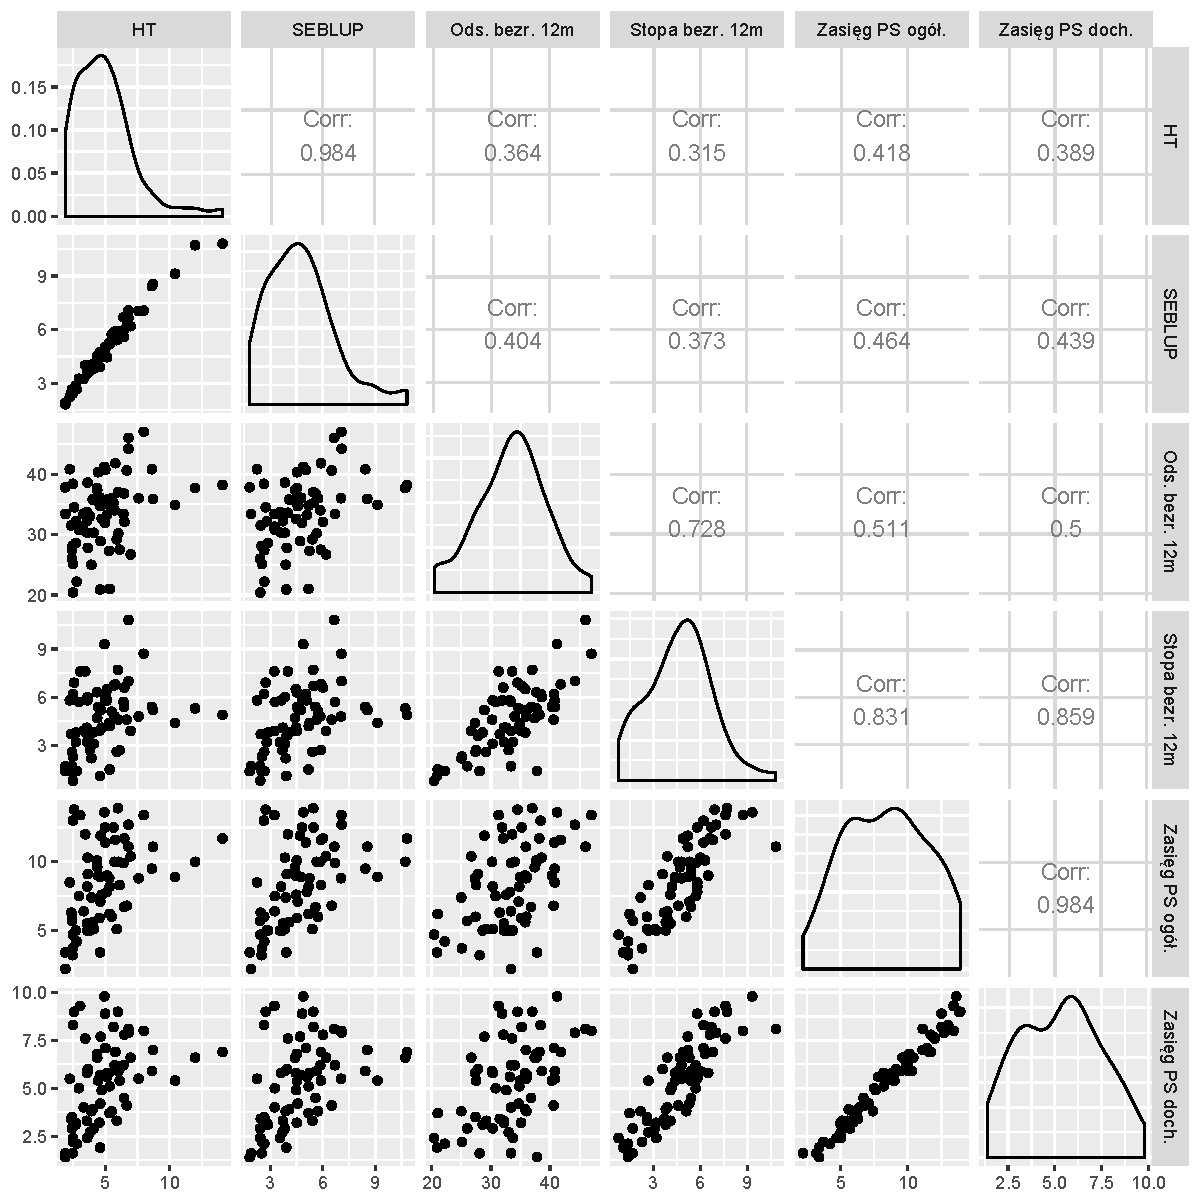
\includegraphics[width=0.8\textwidth]{05_wykresy/pgi_podreg_por-1.pdf}\\
\small{Źródło: opracowanie własne na podstawie EU-SILC 2011 oraz BDL.}
\label{fig:pgi_podreg_por}
\end{figure}

\begin{figure}[ht]
\caption{Porównanie oszacowań głębokości ubóstwa z danymi pochodzącymi z rejestrów administracyjnych na poziomie powiatów}
\centering
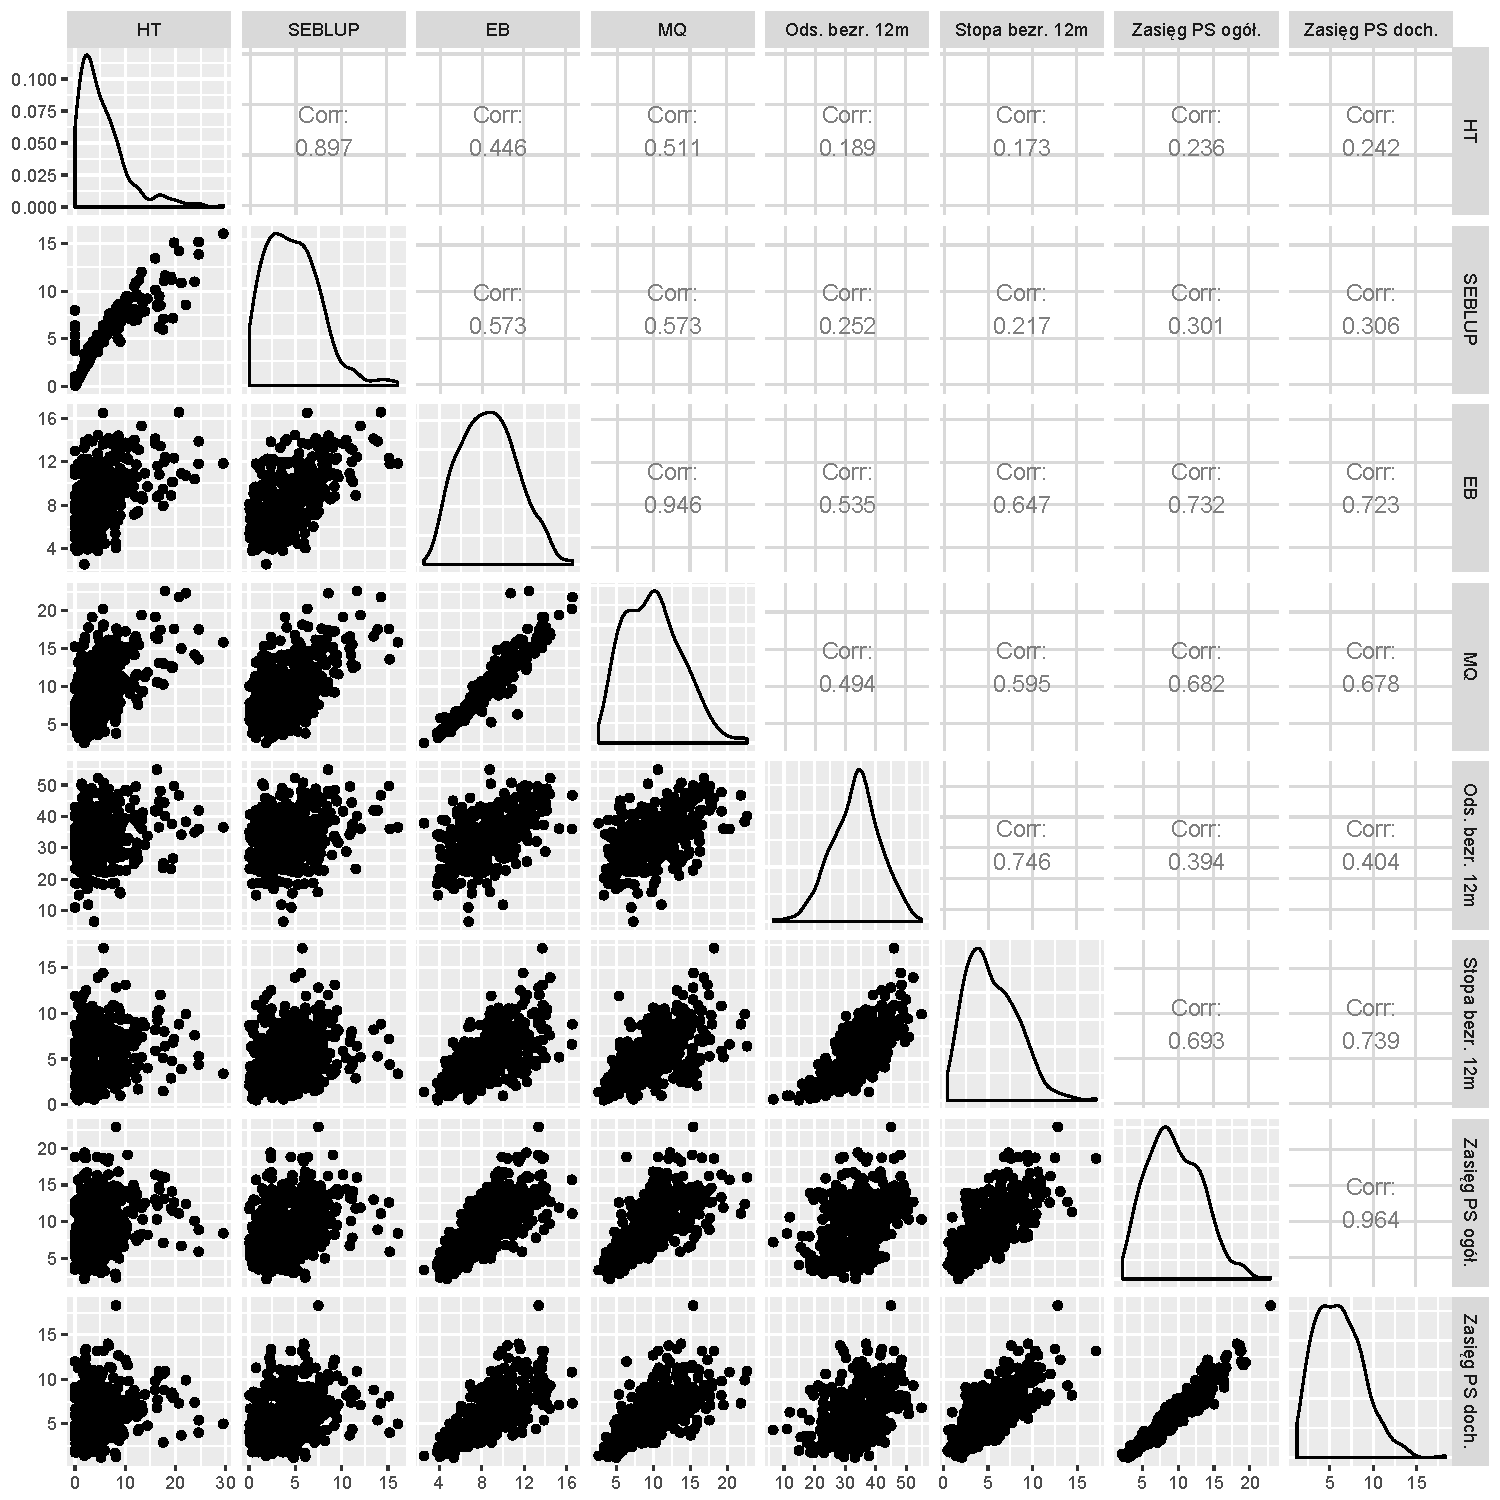
\includegraphics[width=0.8\textwidth]{05_wykresy/pgi_pow_por-1.pdf}\\
\small{Źródło: opracowanie własne na podstawie EU-SILC 2011, NSP 2011 oraz BDL.}
\label{fig:pgi_pow_por}
\end{figure}

